			
%%%%%%%%%%%%% 6 %%%%%%%%%%%%%	
\chapter{Results of Analysis Cuts, Candidates, Backgrounds, and Limits}
%%%%%%%%%%%%%%%%%%%%%%%%%%%%%
	Using the methods, cuts, and a priori determined cut values described in the previous chapter, a set of final CR candidates was determined.

\section{Results of Impulsivity Analysis Cuts}
		After making the impulsivity cuts on the quality event dataset, only 5997 events remain.  This represents $1.44\times10^{-4}$ of the initial Hpol triggered dataset.  Table \ref{tab:weakCutReason} describes the number of events that failed each reduced quantity.
		
		\begin{figure}
		\centering
		\begin{tabular}[c]{|l|c|c|c|}
		\hline
		Cut Parameter & Events Failed & Events Failed \\
		 & (Single) &  (Cumulative) \\
		\hline
		Map Peak & 2238151 & 2238151 \\
		Map SNR & 2247560 & 25364    \\
		Hilbert Peak & 2056059 & 39710    \\
		Linear Polarization Fraction & 2356046 & 90502   \\
		Coherent Template Correlation & 2380525	& 12160    \\
		Deconvolved Template Correlation & 2318737 & 738	   \\
		\hline
		\end{tabular}
		\caption{The number of events removed by each impulsivity cut from the set of events that has already been reduced with quality cuts, mentioned in Table \ref{tab:qualityCutReason}.  The cuts remove any event with a single value below those in Table \ref{tab:cutValues}.  The column marked Single is the number of events that fail that specific cut parameter if applied to all the data.  The column marked Cumulative is if each cut was taken sequentially, and the event removed if failing, before moving to the next.  The final column is the remaining number of events after each cut.}
		\label{tab:weakCutReason}
		\end{figure}
		

	
	\subsection{Above horizon events}
		Of the events that pass the impulsivity cuts, 641 occur above the horizon and do not trace back to the continent, but are below zero elevation.  Included in this set would be CRs interacting in the atmosphere being observed directly.  These events cannot be clustered in the same way as events that land on the continent.  Since they are individual observations from a single location, there is no ability to use parallax to determine their source location depth.  Because of this, a method of temporal and pointing clustering is used to determine if they are part of the same source distribution.  This is not done until the final signal cuts are made.
		

	\subsection{Event pointing results}
		Of the 5356 events that point below the horizon, when compared against themselves, only 32 fall at least $L>40$ away from any other event in the set. This clustering result is shown in Figure \ref{fig:clusteredImpulsives}.  These events are impulsive in nature, and contain the final candidate set.
		
		\begin{figure}
			\centering
				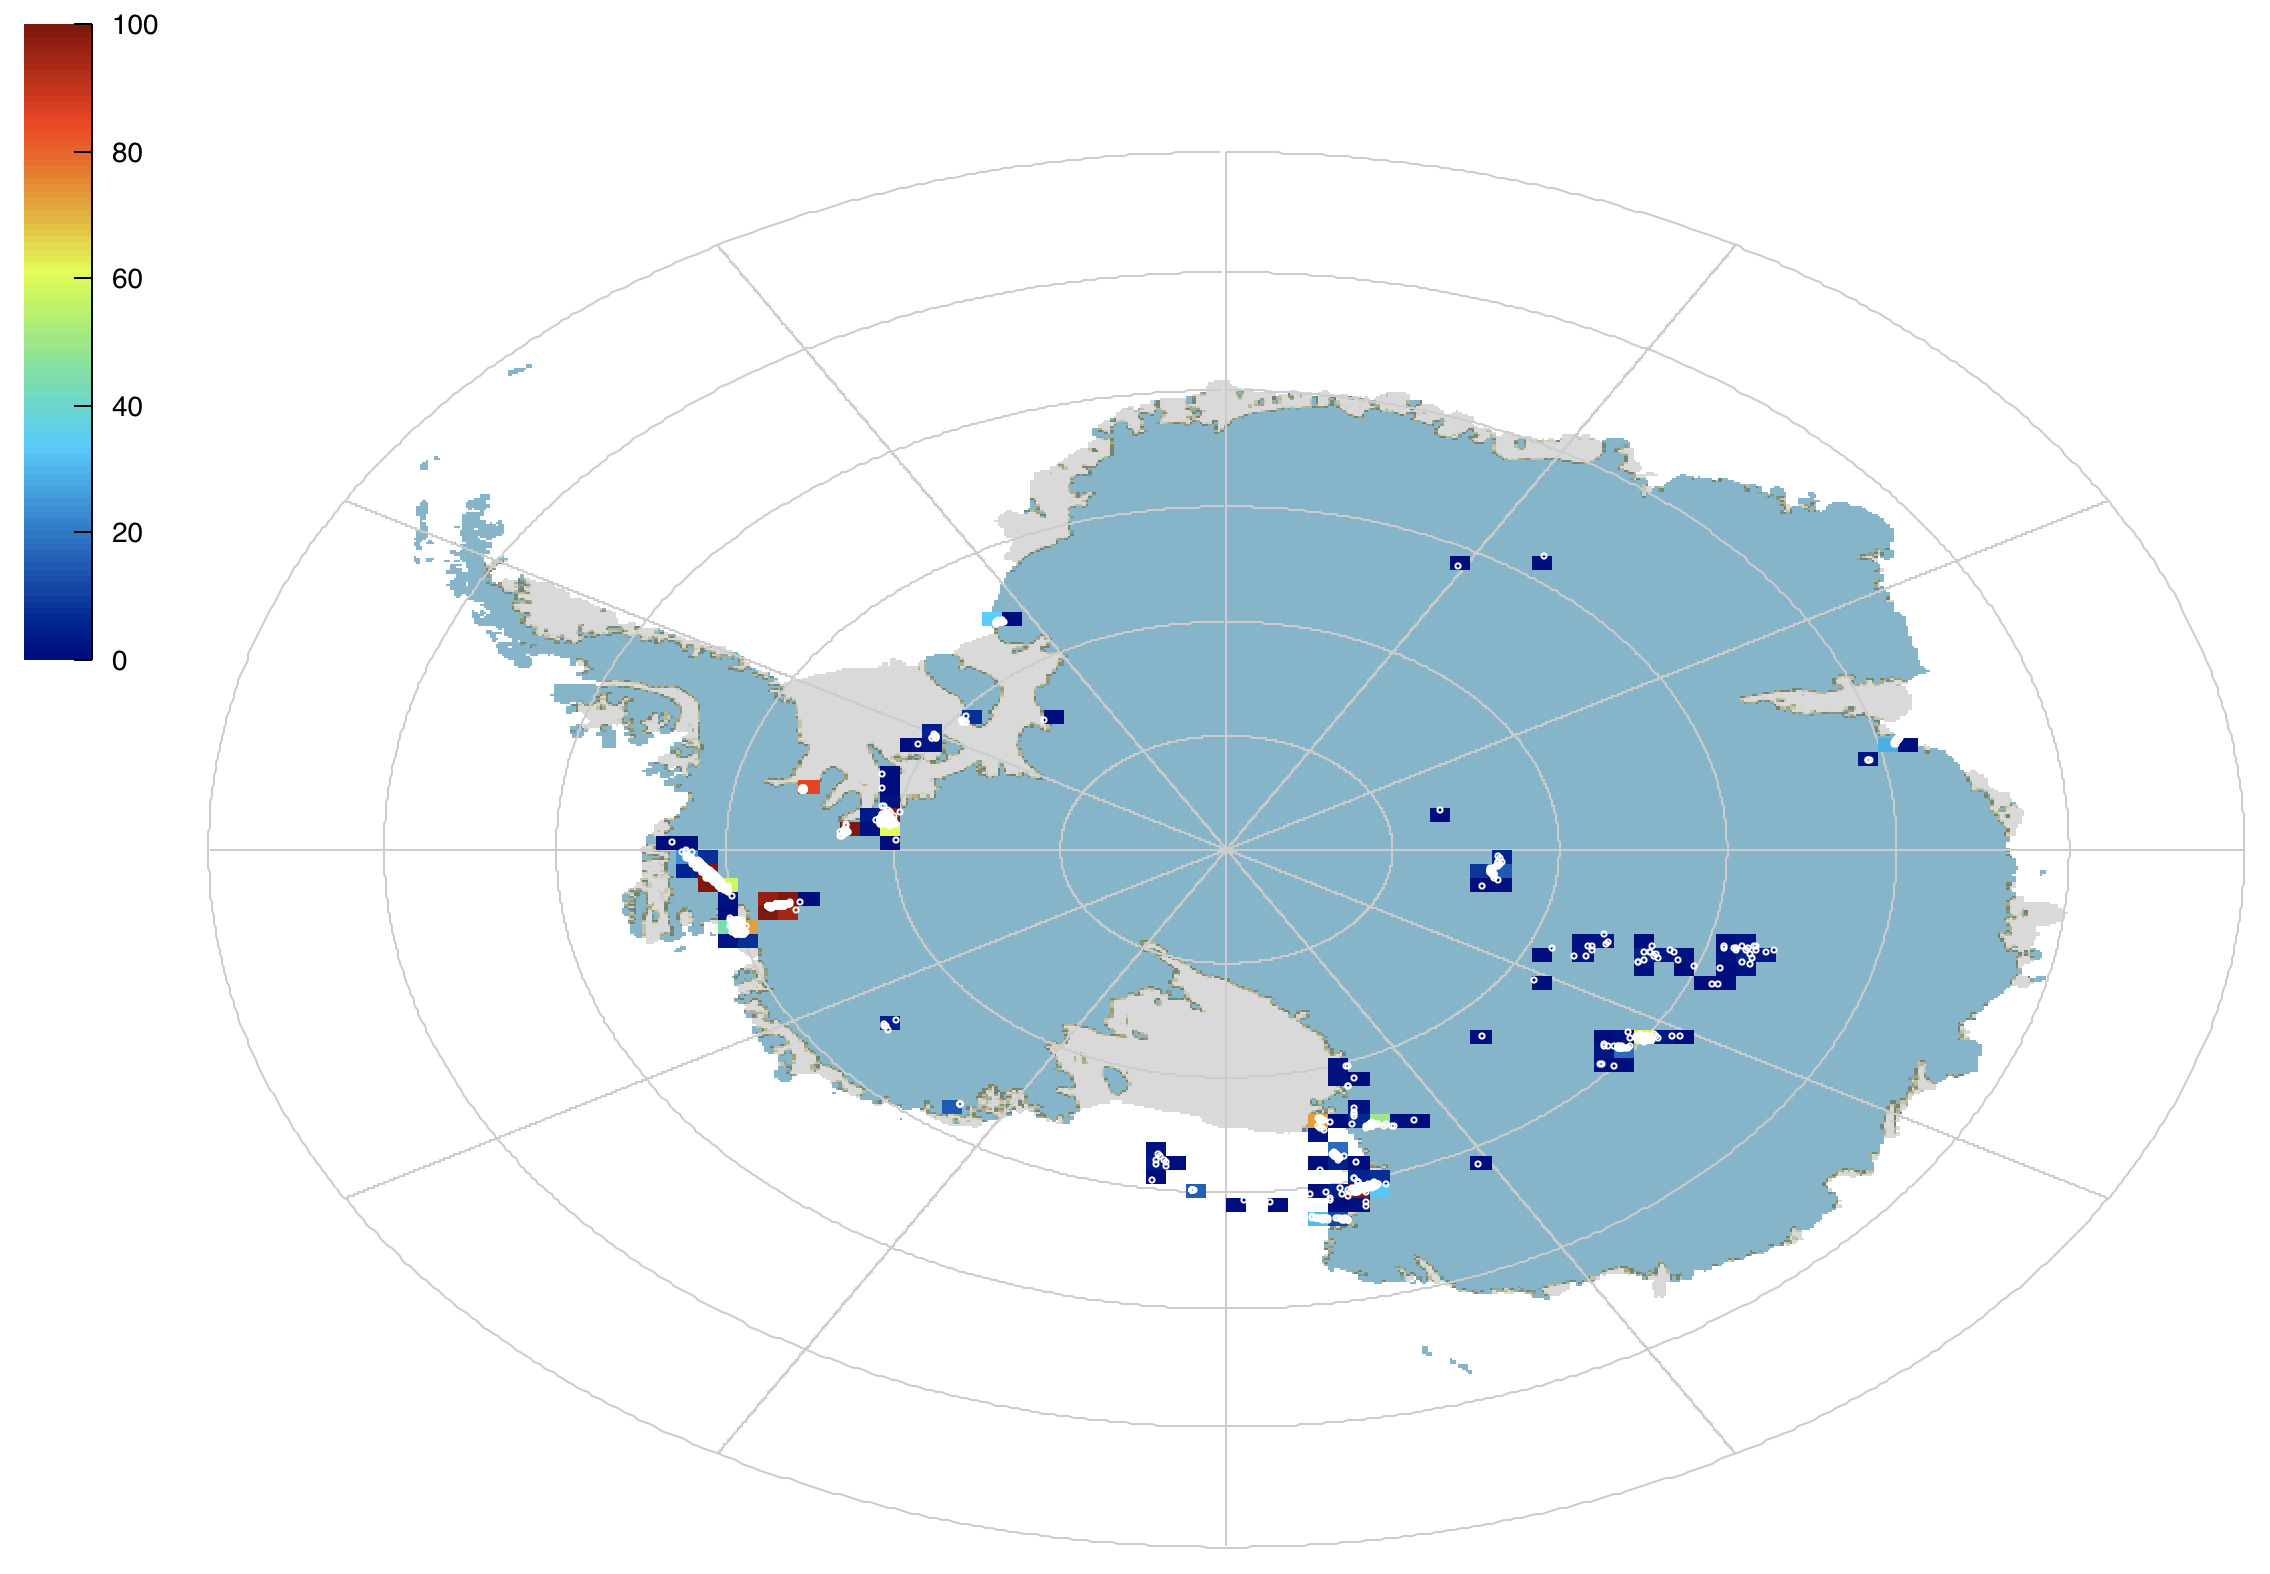
\includegraphics[width=\textwidth]{figures/clusteredImpulsives}
				\caption{A 2D histogram overlaid on a map of Antarctica, showing the locations of the 5324 clustered events.  White circles denote the location of an event that was determined to have clustered.  Events are only required to have one other event with $L<40$ to count as a cluster.  The Z axis shows the number of events that fall into each bin.} 
			\label{fig:clusteredImpulsives}
		\end{figure}	
	

%	\subsection{Pseudo-base locations}
%		The locations where events do cluster can be separated into various pseudo-base locations.  These locations can be seen in Figure \ref{fig:pseudoBases}.  These regions will later be used to derive the expected distributions from impulsive signal producing bases.  The extent of these cluster distributions and the areas of the continent the exclude can be used to determine the overall exposure of the instrument.
%		
%		\begin{figure}
%			\centering
%				\includegraphics[width=\textwidth]{figures/pseudoBases}
%				\caption{A map of Antarctica showing the locations of clustered events and isolated impulsive events.} 
%			\label{fig:pseudoBases}
%		\end{figure}	

\section{Results of Signal Analysis Cuts}
		Making the final CR signal cuts on the weak event list, regardless of clustering status, yields 882 events.  873 of these project onto the continent, and 9 point above the horizon.  Of the nine that point above the horizon, 7 can be removed due to either clustering with events that fall at the horizon, temporal and true azimuth clustering.  These removed events, and the clusters they associate to, can be found in Table \ref{tab:aboveHorizonClustering}. The below horizon CR candidates can be determined by choosing events within this, and results in 18 downward pointing CR candidate events, and 2 events within the atmosphere, for 21 events total.  
		
	\begin{figure}
		\centering
		\begin{tabular}[c]{|l|p{7cm}|}
		\hline
		Event Number Removed & Clustering description \\
		\hline
		48160214 &  Clusters with other events on the continent with 0.12 downward $\theta$ adjustment \\
		\hline
		58112462 &  Clusters with other events on the continent with 0.02 downward $\theta$ adjustment \\
		\hline
		69050305 &  Cluster with other points on the continent with  $<0.1^\circ$ downward $\theta$ adjustment \\
		69050312 &  \\
		69050331 &  \\
		\hline
		80134362 &  Part of a 401 above horizon event burst lasting 624 seconds. Event numbers 79995831 - 80745194. \\
		80299371 &  \\
		\hline
		\end{tabular}
		\caption{Above horizon clusters that contain events that pass final signal cuts.  7 events are excluded from the final candidate list due to events in close time proximity, pointing in the same direction.}
		\label{tab:aboveHorizonCluster}
	\end{figure}
	
	
		
		Table \ref{tab:signalCutReason} describes the number of events from the impulsive set that failed each reduced quantity.  Note that interferometric map peak and map SNR do not change between the cuts, so they are not included in this table.
		
		\begin{figure}
		\centering
		\begin{tabular}[c]{|l|c|c|}
		\hline
		Cut Parameter & Events Failed & Events Failed \\
		 & (Single) &  (Cumulative) \\
		\hline
		Hilbert Peak & 147 & 147\\
		Linear Polarization Fraction & 3060 & 2948\\
		Coherent Template Correlation & 4179 & 1920\\
		Deconvolved Tempalte Correlation & 4265 & 97\\
		\hline
		\end{tabular}
		\caption{}
		\label{tab:signalCutReason}
		\end{figure}
		
		
	\subsection{Candidate locations on continent}
		The locations of the final 18 below horizon and 2 above horizon candidates can be seen in Figure \ref{fig:downwardEventMap}.
		
			\begin{figure}
			\centering
				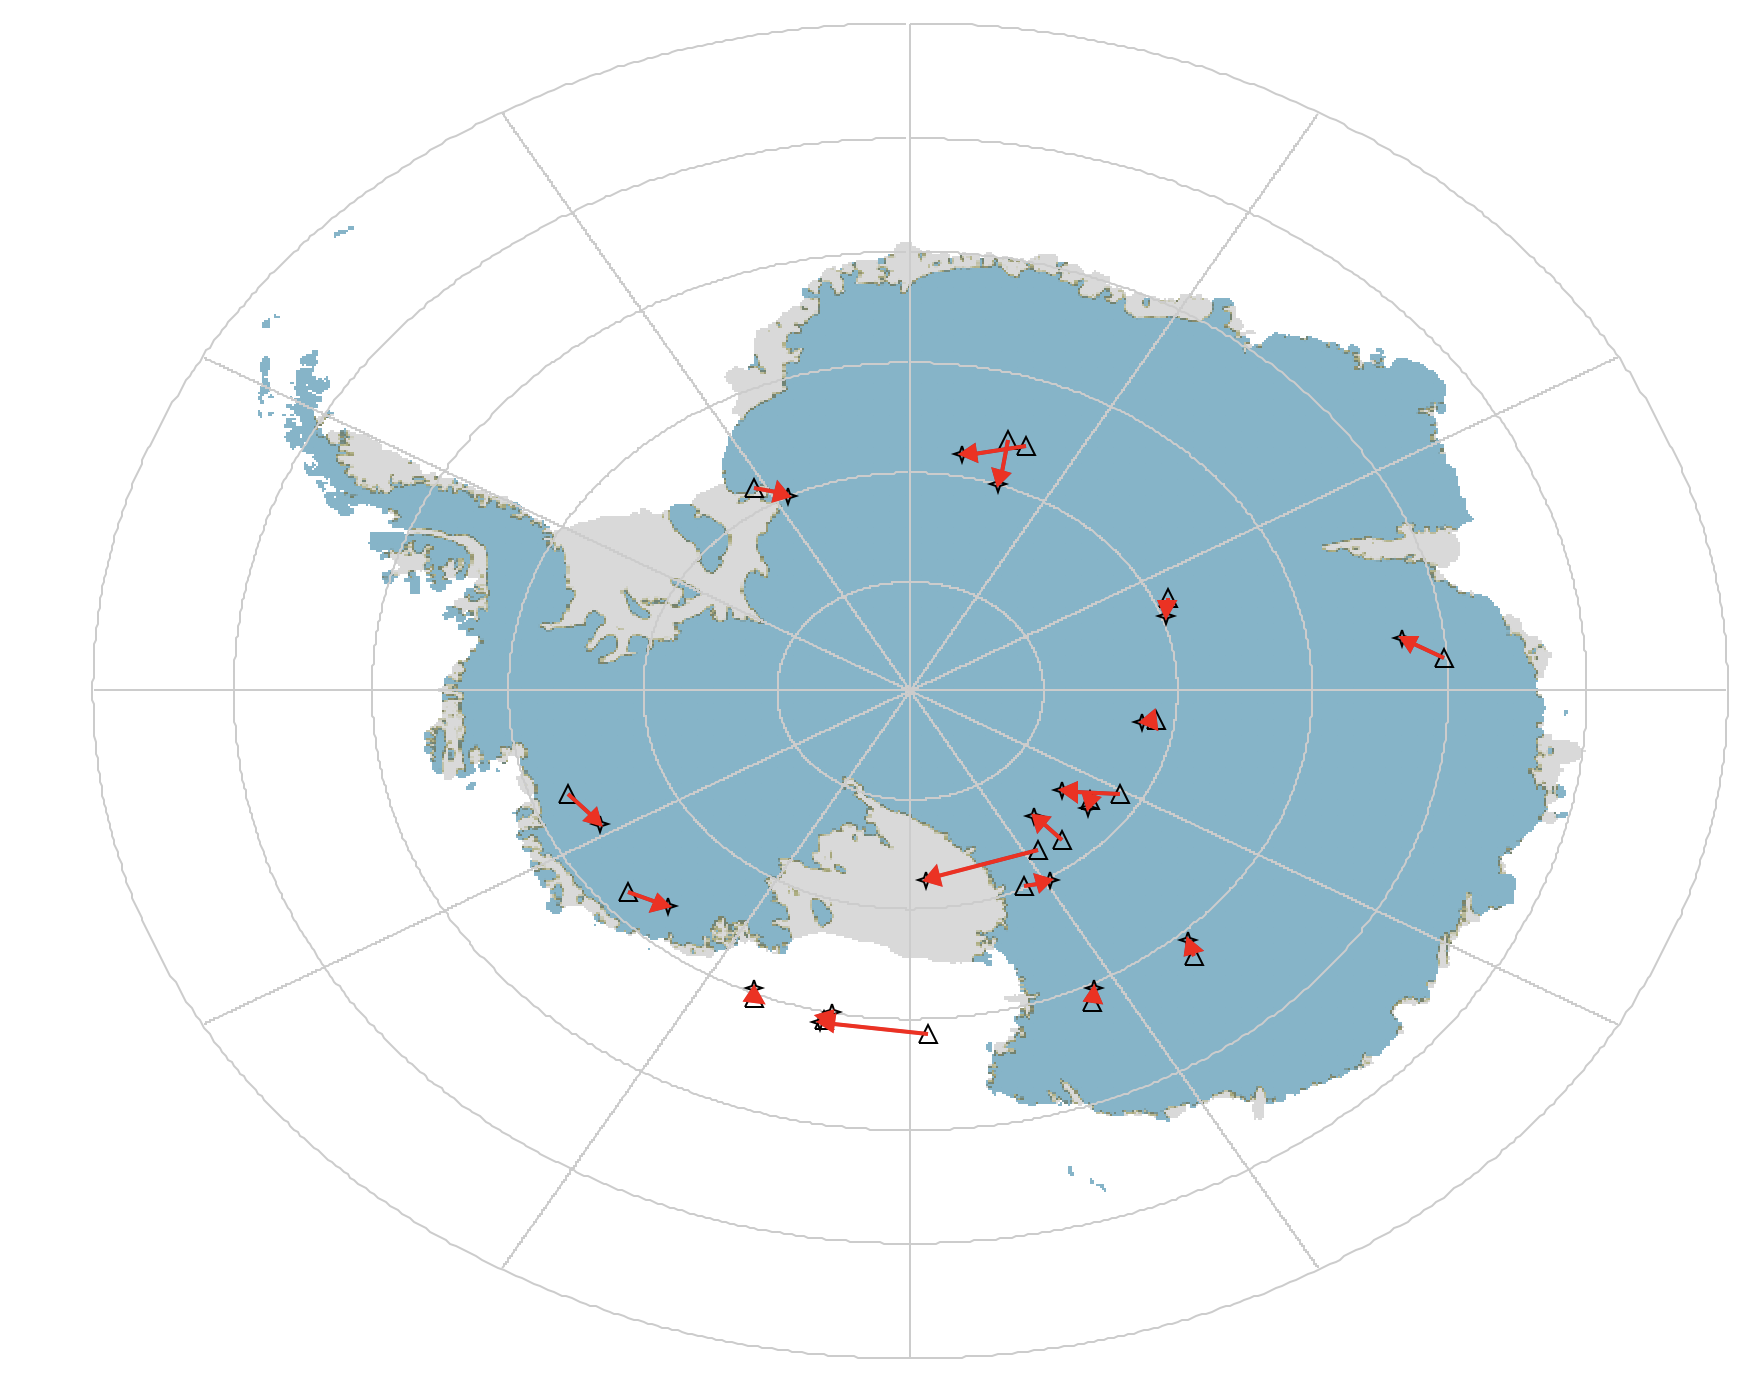
\includegraphics[width=\textwidth]{figures/downwardEventMap}
				\caption{Locations of the CR candidate events discovered in the analysis.  The triangle is the location of ANITA, the X denotes the location on the continent where the event traces, and arrow is the vector between the two.  Above horizon events, which do not project to the continent, are shown with blue arrows indicating their observation direction.}
			\label{fig:downwardEventMap}
			\end{figure}		

\section{Background Estimates}
	\label{sec:backgroundEstimate}
	Estimating the number of background events that passed all signal cuts and are present in the final candidate list is import for establishing the confidence in the final result.  The strong cut on the 

\section{Diffuse Source Frequentist Background Estimate}
	 This is accomplished using statistical inference about the probability that non-physics events would satisfy all cut requirements~\cite{ClassicalStatisticalEstimation}.  We attempt to divide the events into two sets, one background and one signal, then use the arithmetic of probability to determine the likelihood that an event from the background set could be found within the signal set.  

	In order to relate the measured data to uniform 
	
	Bayes' theorem is stated in Equation \ref{eqn:bayesTheorem}, and can be used to determine the estimate of the background.

	\begin{equation}
		P(B | S) = \frac{P(S | B) P(B)}{P(S)}
	\label{eqn:bayesTheorem}
	\end{equation}
	
	Where P(B) is the number of events in the background set
	
	
	Two different philosophies can be referenced for determining what goes into the background set.  The signal set can be defined as either the expected observation rate of UHECR particles during the flight, or as a single count for each measured candidate event individually which is then summed to find the total background probability.
	
	\subsection{Frequentist Probability}
		%I think Abby's suggested method, simply taking the ratio of impulsive events passing cuts and clustering to all clustered events regardless of impulsivity,  is Frequentist for sure, since it relies only on observed transient producing locations.  
		
		
\section{Local Frequentist Background Estimate}
	



%\section{ABCD Background Estimate}
%		The ABCD method is a common particle physics background estimator in which the ratio of background event populations within two areas of parameter space, combined with the number of events with characteristics placing it in a third, neighboring, space, can be used to derive the expected background count in a signal box region.  This expected background can then be compared versus the number of events that are actually seen to occur within that signal box.  Assuming that the distribution is constant throughout the four regions for background, and that signal only lies within the signal box, any upward deviation from the expected background count can be assumed to be the signal.
		
%		This method presents issues 
		

\section{Cosmic Ray Candidate Results}
	There were 18 events that passed all signal cuts and did not cluster to any other impulsive event on the continent, and are hereby known as the cosmic ray candidates.  Of these 18, 2 point above the horizon but still within the atmosphere, indicating that they are directly viewed EAS signals that do not reflect off the continent.  The remaining 16 point downwards and project onto the continent.  These events, their waveforms, their locations on the continent, and the distributions of nearby events  are presented in the following section.  A map summarizing the results of the analysis, including the locations of the events on the continent, along with events that cluster and events that pass impulsivity cuts but fail signal cuts, is shown in Figure \ref{fig:allEventsMap}. An overlay of measured horizontally polarized waveforms for all candidates, aligned to their peak correlation and polarity flipped relative to their estimated polarity, is shown in Figure \ref{fig:hPolOverlay}.  The vertically measured waveforms have significantly less signal but are presented with alignment determined through H-Pol correlation in Figure \ref{fig:vPolOverlay}.  Additionally, the coherently summed waveforms are presented side by side in figure \ref{fig:allCandidates_coherent}.
	
		\begin{figure}
			\centering
				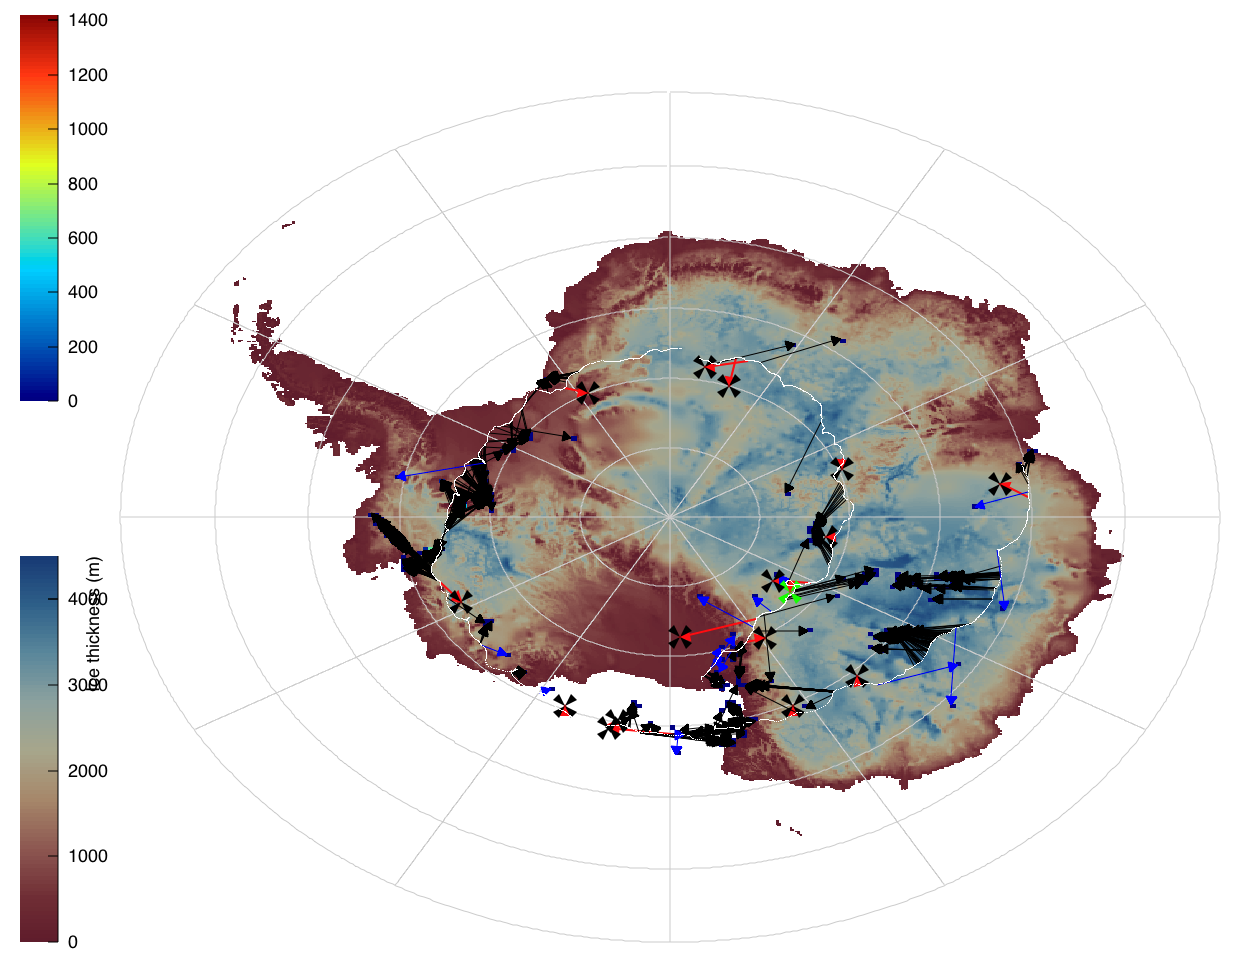
\includegraphics[width=\textwidth]{figures/allEventsMap}
				\caption{A map of Antarctica summarizing the results of the analysis.  "X"s with red arrows denote the mapped location on the continent for the 18 CR candidates.  The blue arrows show locations of isolated events that did not meet signal cuts.  The black arrows and underlaying histogram shows events that were discovered with the impulsivity cuts, but failed either signal cuts or clustering cuts. } 
			\label{fig:allEventsMap}
		\end{figure}		
		
		\begin{figure}
			\centering
				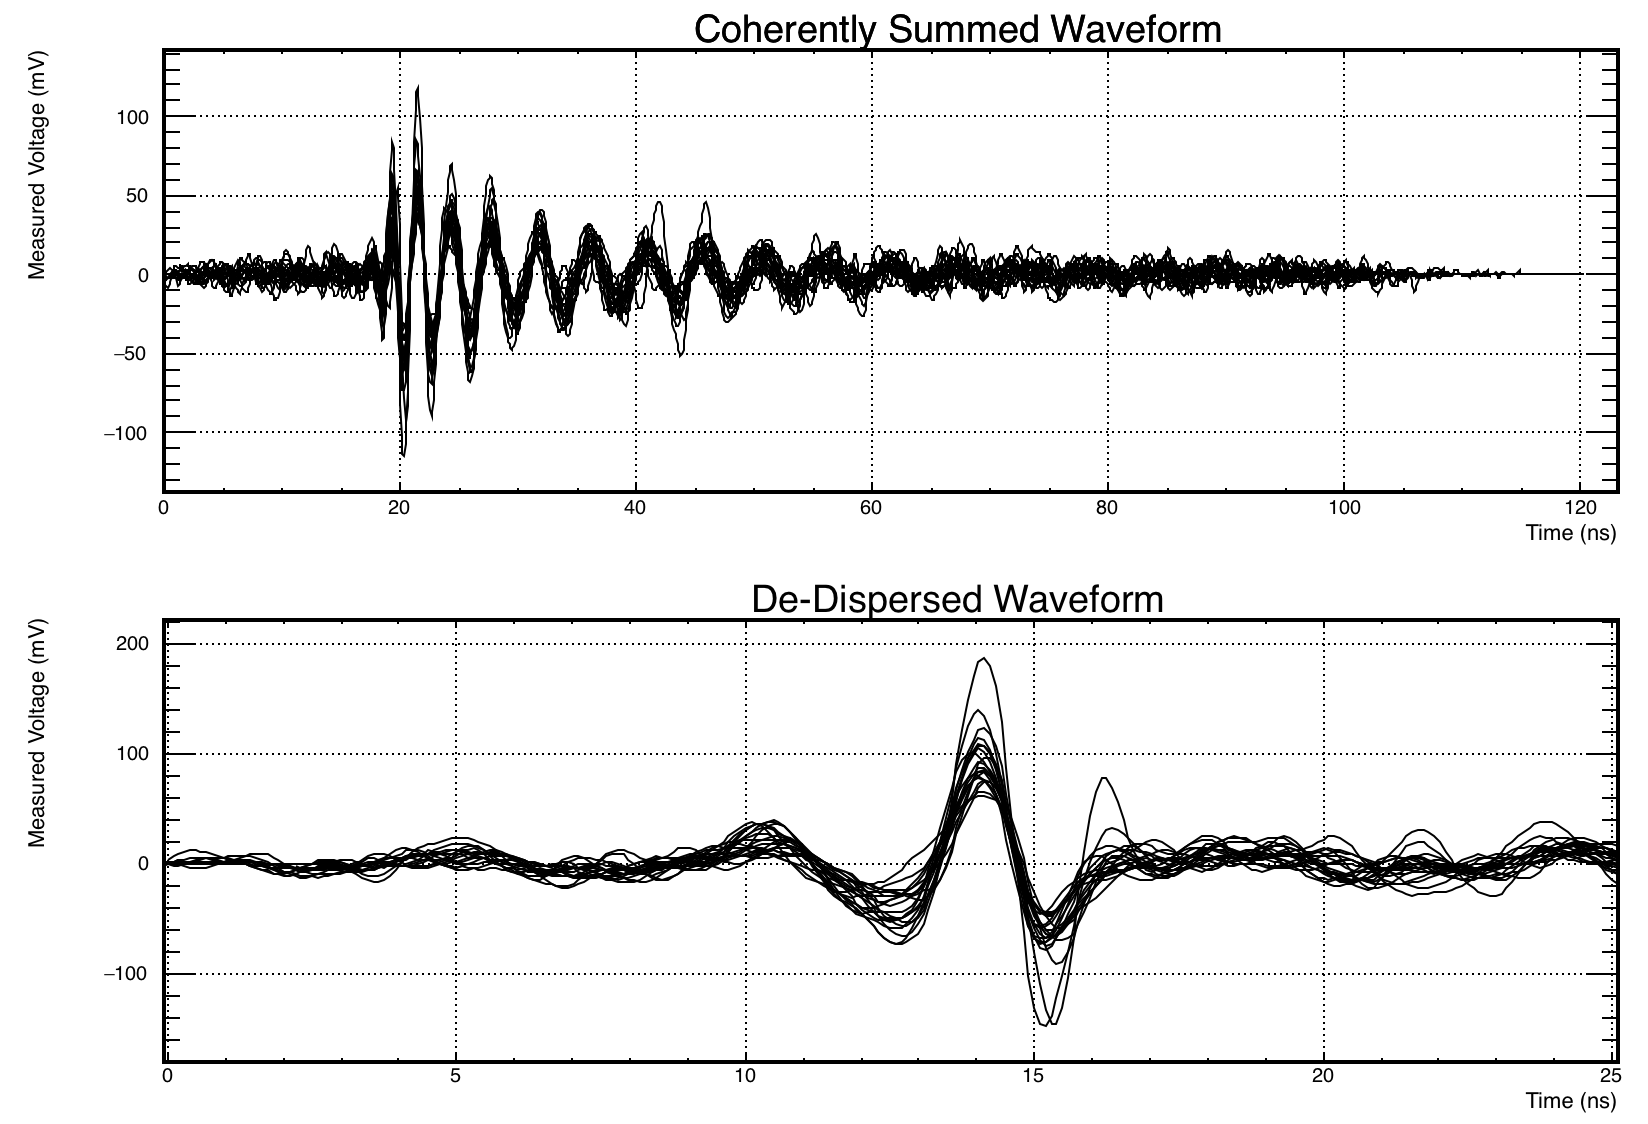
\includegraphics[width=\textwidth]{figures/hPolOverlay}
				\caption{All 20 CR candidate H-pol measured signals events overlaid.  Their blinded polarity has been aligned with respect to their estimated polarity.  They have aligned to their peak correlation.  Top: Coherently summed waveform.  Bottom: All Pass Filter De-dispersed waveform. } 
			\label{fig:hPolOverlay}
		\end{figure}
		
		\begin{figure}
			\centering
				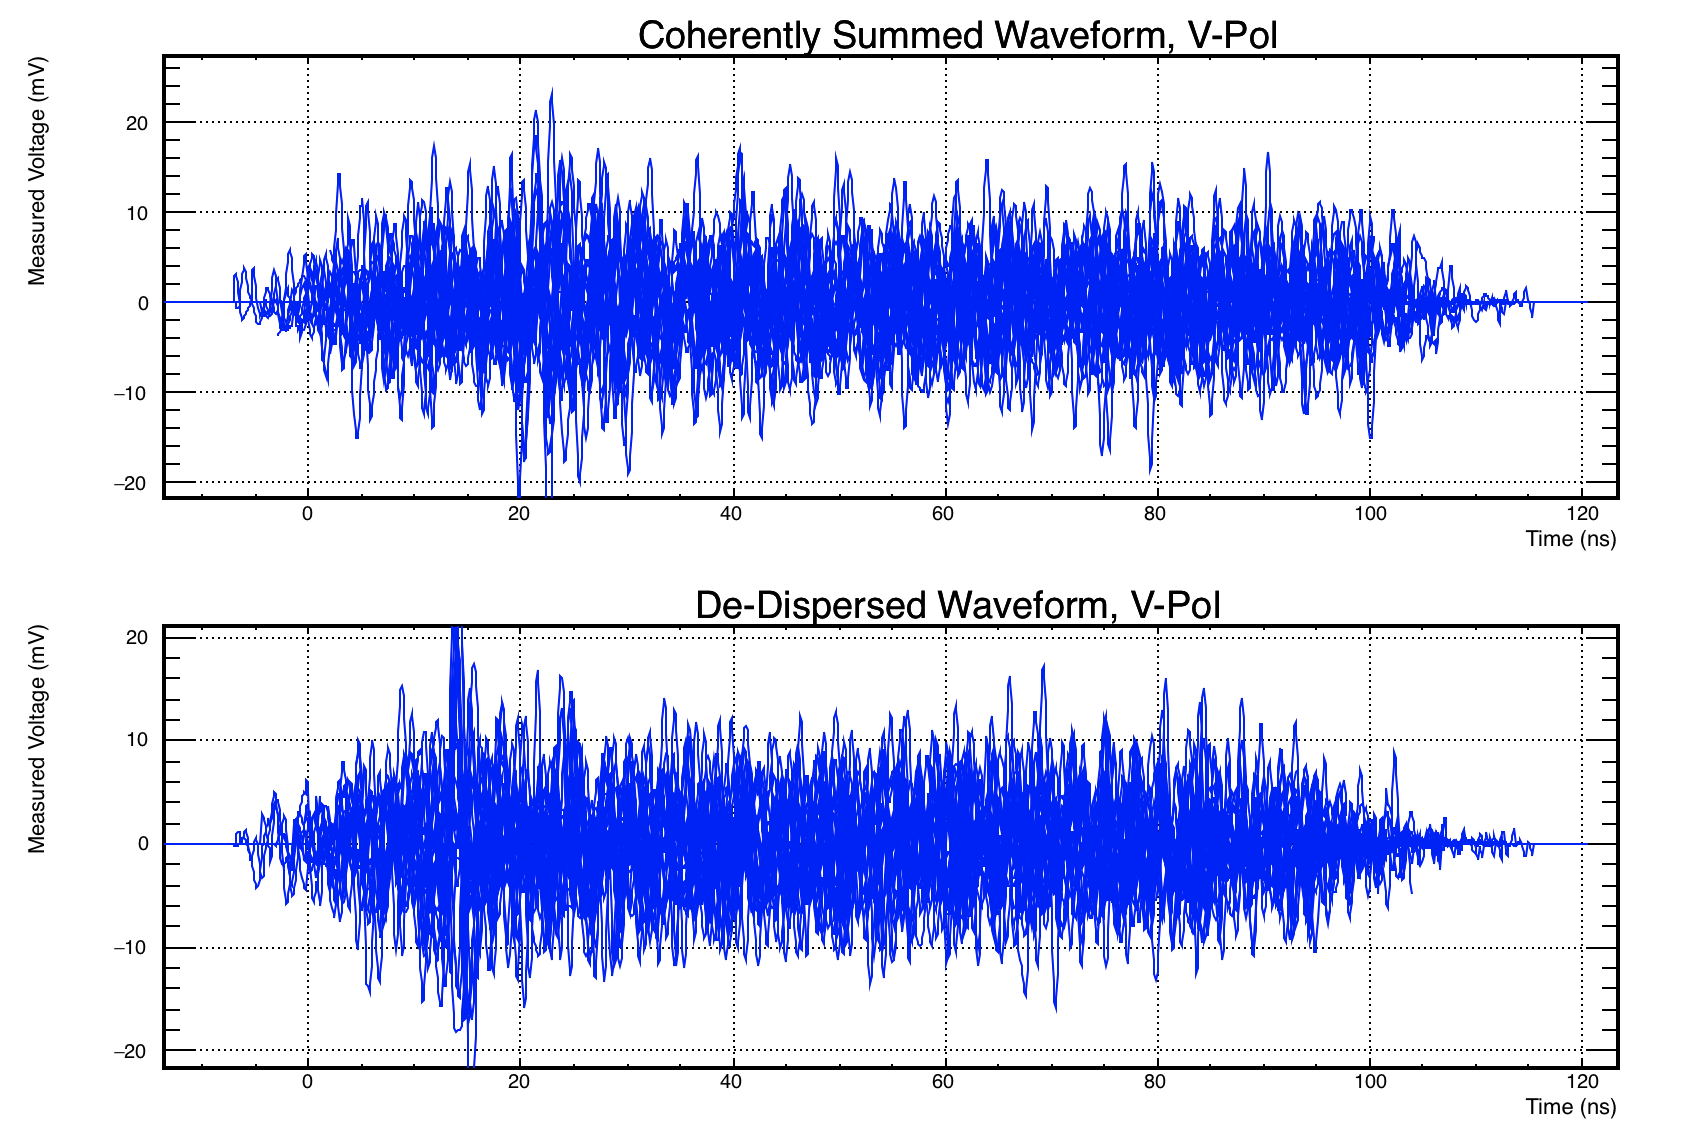
\includegraphics[width=\textwidth]{figures/vPolOverlay}
				\caption{All 20 CR candidate V-pol measured events overlaid.  They are aligned to the peak of the correlation of the H-pol signal, which has significantly more power.  The amount of signal expected in this polarization is dependent on location in the geomagnetic field, and the incidence angle of the UHE particle.  Top: Coherently summed waveform.  Bottom: All Pass Filter De-dispersed waveform. } 
			\label{fig:vPolOverlay}
		\end{figure}	
	
		\begin{figure}
			\centering
				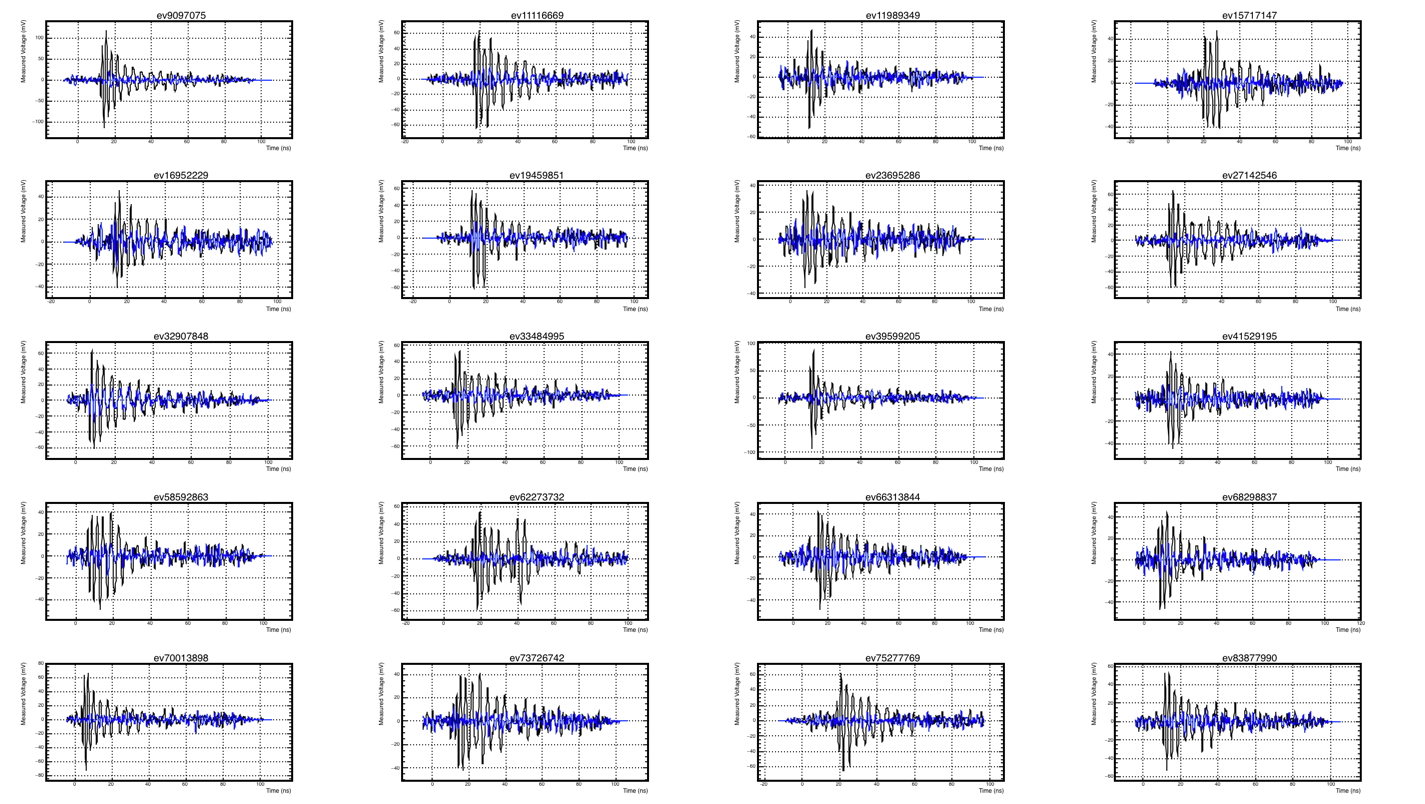
\includegraphics[width=\textwidth]{figures/allCandidates_coherent}
				\caption{All 20 CR candidate events.  Their blinded polarity has been aligned with respect to their estimated polarity. Black lines denote the H-Pol signal, while blue lines denote the V-Pol signal. } 
			\label{fig:allCandidates_coherent}
		\end{figure}		
			
	
	
	
	\subsection{Direct events}
		There were 2 events that were observed above the horizon, but still within the atmosphere.  Summaries of each of their characteristics are provided below.	
		\subsubsection{Event 27142546}
			\begin{figure}
			\centering
				\includegraphics[width=\textwidth]{figures/eventStuff/Ev27142546_waveform}
				\caption{Top Coherently summed waveform.  Bottom: De-dispersed waveform} 
			\label{fig:Ev27142546_waveform}
			\end{figure}		

		\begin{figure}
		\centering
			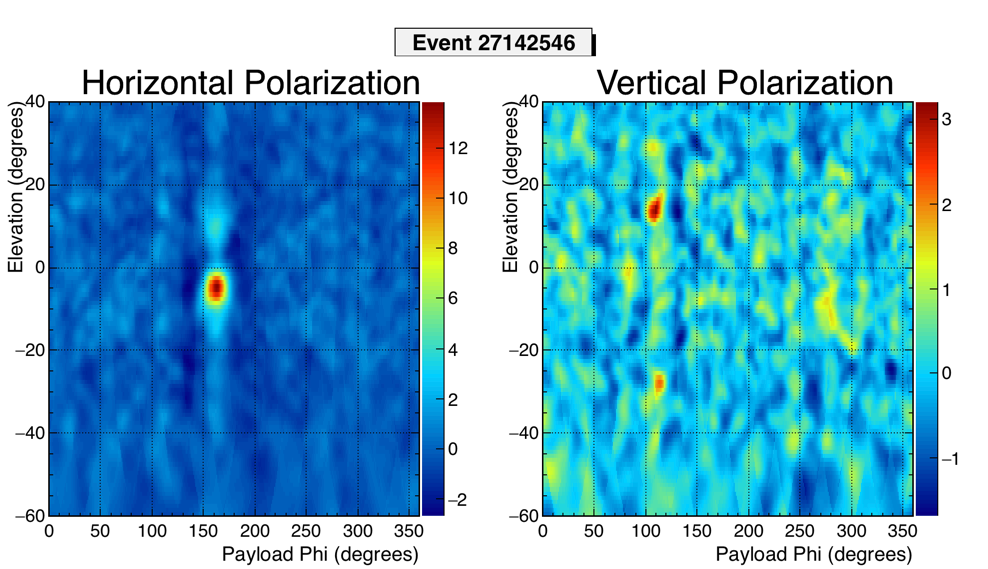
\includegraphics[width=\textwidth]{figures/intMap/intMap_ev27142546}
			\caption{Interferometric maps for event 27142546} 
		\label{fig:Ev27142546_map}
		\end{figure}			
			
				\subsubsection{Event 39599205}
			\begin{figure}
			\centering
				\includegraphics[width=\textwidth]{figures/eventStuff/Ev39599205_waveform}
				\caption{Top Coherently summed waveform.  Bottom: De-dispersed waveform} 
			\label{fig:Ev39599205_waveform}
			\end{figure}
			
		\begin{figure}
		\centering
			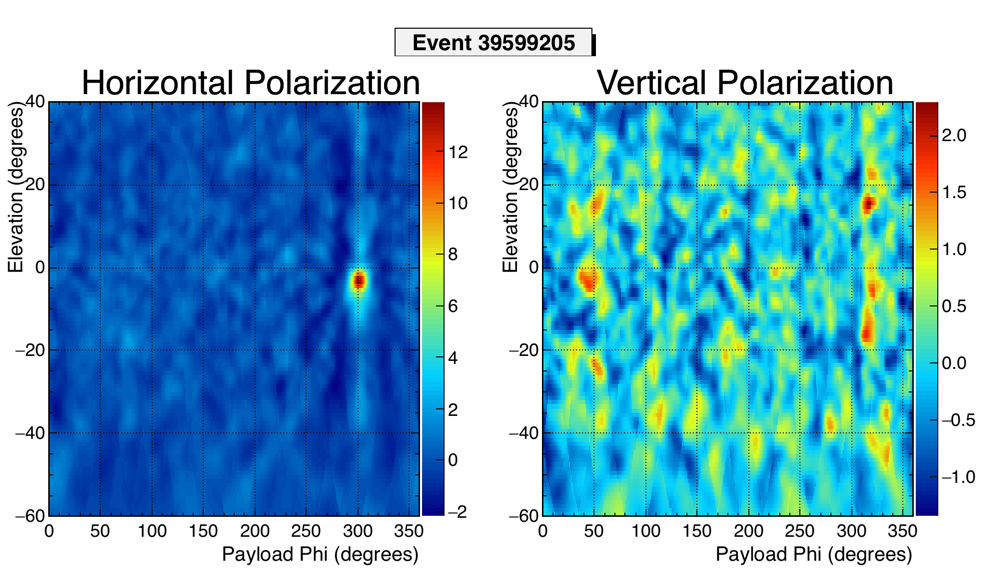
\includegraphics[width=\textwidth]{figures/intMap/intMap_ev39599205}
			\caption{Interferometric maps for event 39599205} 
		\label{fig:Ev39599205_map}
		\end{figure}				
		
	\subsection{Reflected events}
		There were 18 events that traced back to the continent.  Summaries of each of their characteristics are provided below.
	
		\subsubsection{Event 9097075}
			Event 9097075 
		
		\begin{figure}
		\centering
			\includegraphics[width=\textwidth]{figures/eventStuff/Ev9097075_waveform}
			\caption{Top Coherently summed waveform.  Bottom: De-dispersed waveform} 
		\label{fig:Ev9097075_waveform}
		\end{figure}

		\begin{figure}
		\centering
			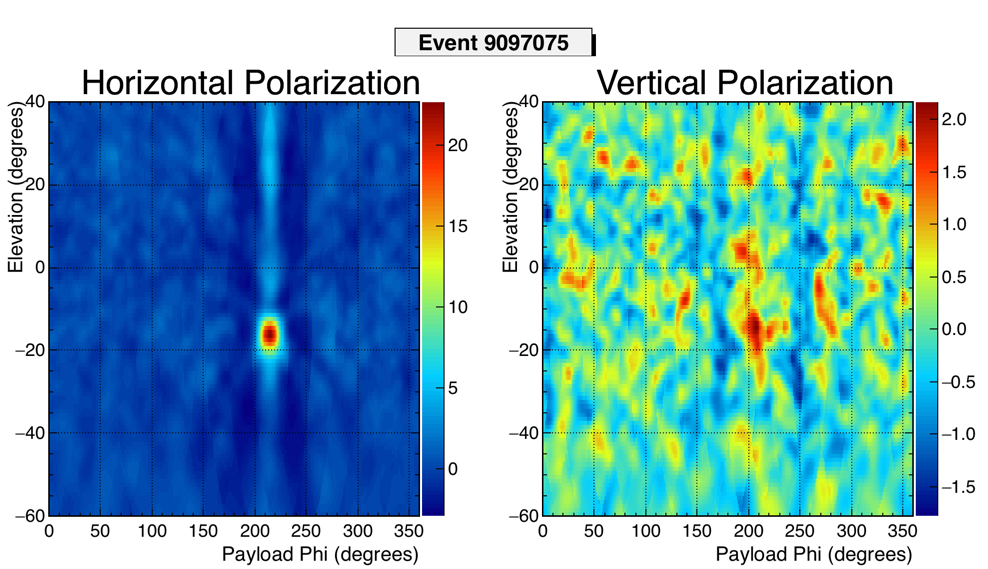
\includegraphics[width=\textwidth]{figures/intMap/intMap_ev9097075}
			\caption{Interferometric maps for event 9097075} 
		\label{fig:Ev9097075_map}
		\end{figure}


		\subsubsection{Event 11116669}
		\begin{figure}
		\centering
			\includegraphics[width=\textwidth]{figures/eventStuff/Ev11116669_waveform}
			\caption{Top Coherently summed waveform.  Bottom: De-dispersed waveform} 
		\label{fig:Ev11116669_waveform}
		\end{figure}
		
		\begin{figure}
		\centering
			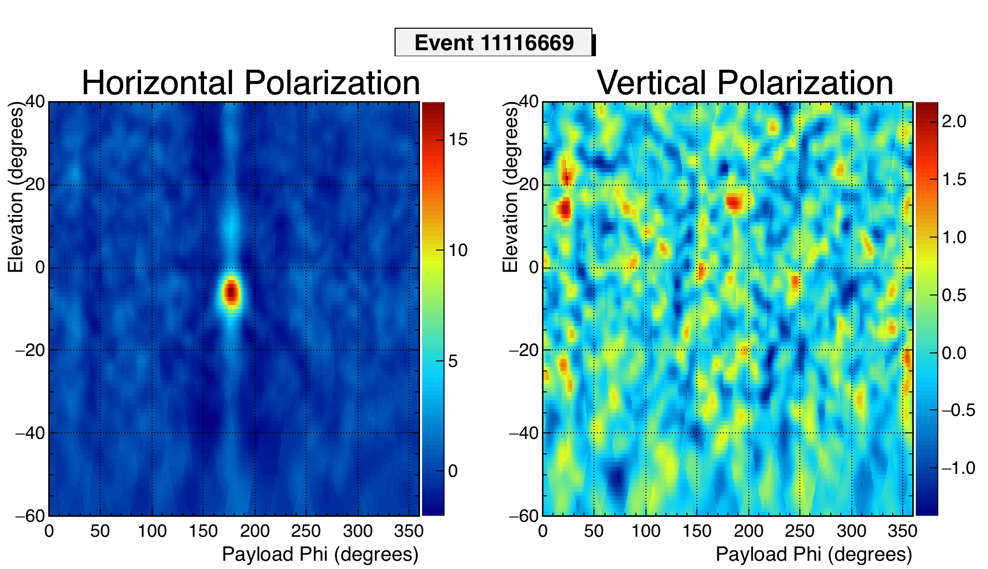
\includegraphics[width=\textwidth]{figures/intMap/intMap_ev11116669}
			\caption{Interferometric maps for event 11116669} 
		\label{fig:Ev11116669_map}
		\end{figure}			
	
		\subsubsection{Event 15717147}
		\begin{figure}
		\centering
			\includegraphics[width=\textwidth]{figures/eventStuff/Ev15717147_waveform}
			\caption{Top Coherently summed waveform.  Bottom: De-dispersed waveform} 
		\label{fig:Ev15717147_waveform}
		\end{figure}
		
		\begin{figure}
		\centering
			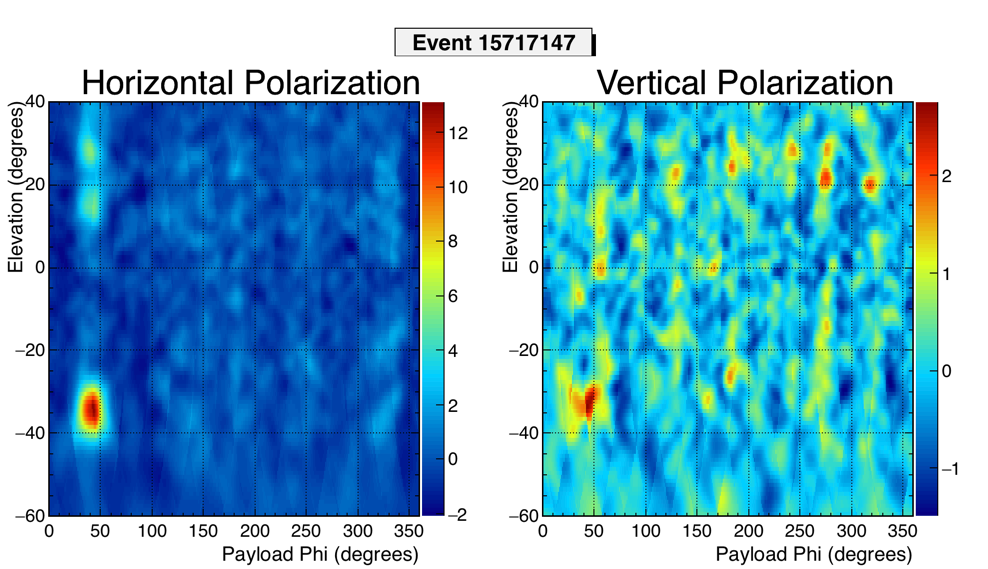
\includegraphics[width=\textwidth]{figures/intMap/intMap_ev15717147}
			\caption{Interferometric maps for event 15717147} 
		\label{fig:Ev15717147_map}
		\end{figure}			
	
		\subsubsection{Event 16952229}
		\begin{figure}
		\centering
			\includegraphics[width=\textwidth]{figures/eventStuff/Ev16952229_waveform}
			\caption{Top Coherently summed waveform.  Bottom: De-dispersed waveform} 
		\label{fig:Ev16952229_waveform}
		\end{figure}
		
		\begin{figure}
		\centering
			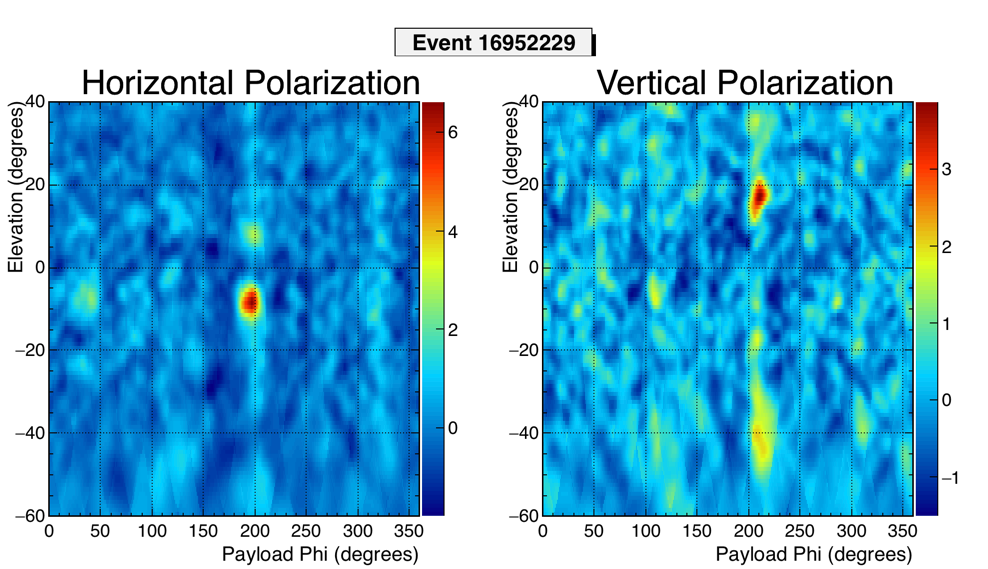
\includegraphics[width=\textwidth]{figures/intMap/intMap_ev16952229}
			\caption{Interferometric maps for event 16952229} 
		\label{fig:Ev16952229_map}
		\end{figure}			
	
		\subsubsection{Event 19459851}
		\begin{figure}
		\centering
			\includegraphics[width=\textwidth]{figures/eventStuff/Ev19459851_waveform}
			\caption{Top Coherently summed waveform.  Bottom: De-dispersed waveform} 
		\label{fig:Ev19459851_waveform}
		\end{figure}
		
		\begin{figure}
		\centering
			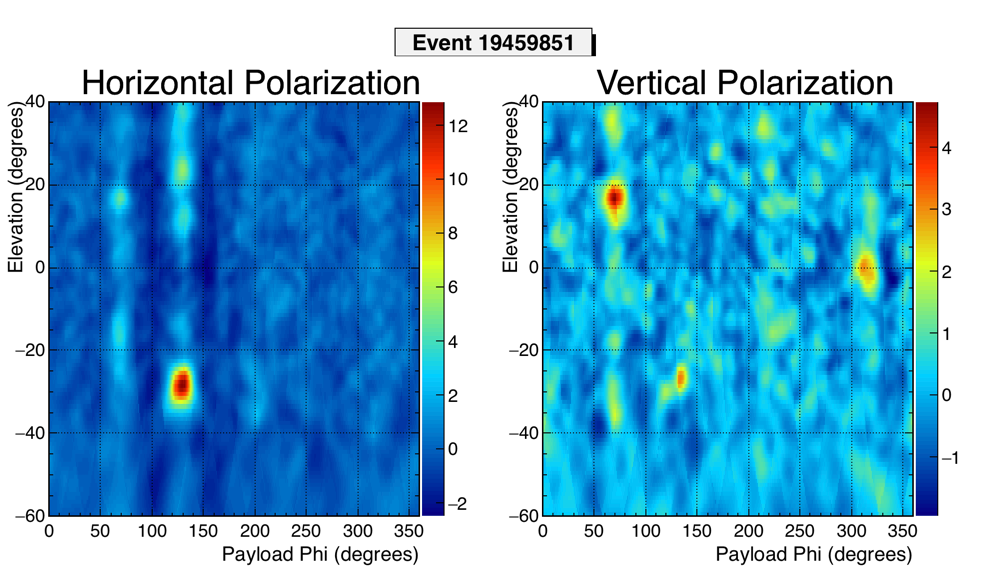
\includegraphics[width=\textwidth]{figures/intMap/intMap_ev19459851}
			\caption{Interferometric maps for event 19459851} 
		\label{fig:Ev19459851_map}
		\end{figure}	
	
		\subsubsection{Event 23695286}
		\begin{figure}
		\centering
			\includegraphics[width=\textwidth]{figures/eventStuff/Ev23695286_waveform}
			\caption{Top Coherently summed waveform.  Bottom: De-dispersed waveform} 
		\label{fig:Ev23695286_waveform}
		\end{figure}
		
		\begin{figure}
		\centering
			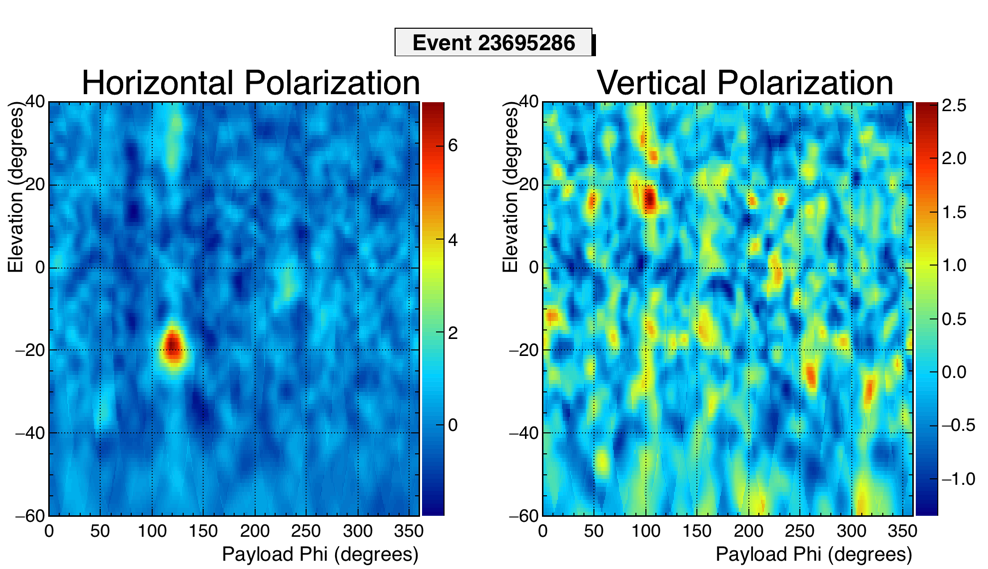
\includegraphics[width=\textwidth]{figures/intMap/intMap_ev23695286}
			\caption{Interferometric maps for event 23695286} 
		\label{fig:Ev23695286_map}
		\end{figure}			
	
		\subsubsection{Event 32907848}
		\begin{figure}
		\centering
			\includegraphics[width=\textwidth]{figures/eventStuff/Ev32907848_waveform}
			\caption{Top Coherently summed waveform.  Bottom: De-dispersed waveform} 
		\label{fig:Ev32907848_waveform}
		\end{figure}
		
		\begin{figure}
		\centering
			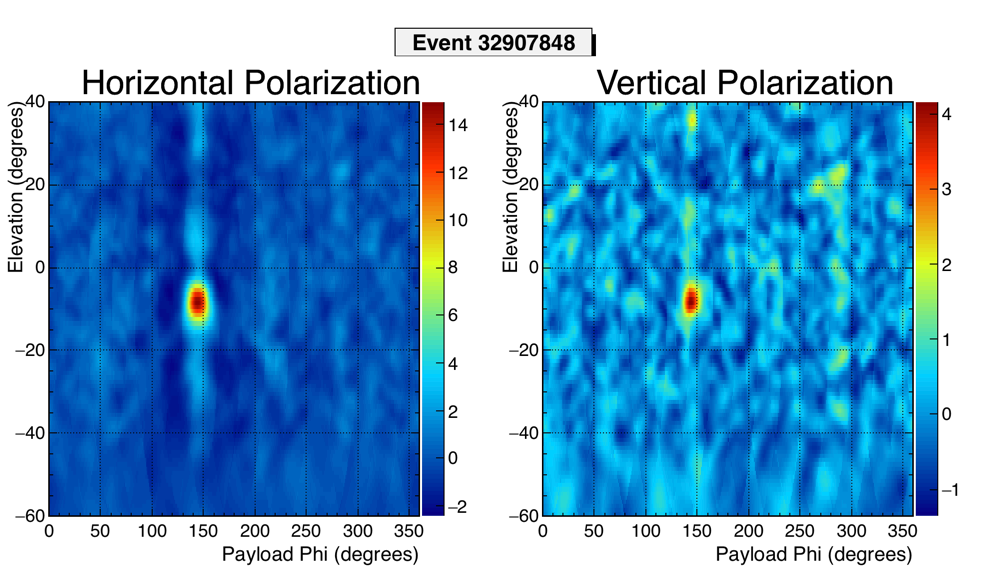
\includegraphics[width=\textwidth]{figures/intMap/intMap_ev32907848}
			\caption{Interferometric maps for event 32907848} 
		\label{fig:Ev32907848_map}
		\end{figure}	
	
		\subsubsection{Event 33484995}
		\begin{figure}
		\centering
			\includegraphics[width=\textwidth]{figures/eventStuff/Ev33484995_waveform}
			\caption{Top Coherently summed waveform.  Bottom: De-dispersed waveform} 
		\label{fig:Ev33484995_waveform}
		\end{figure}
		
		\begin{figure}
		\centering
			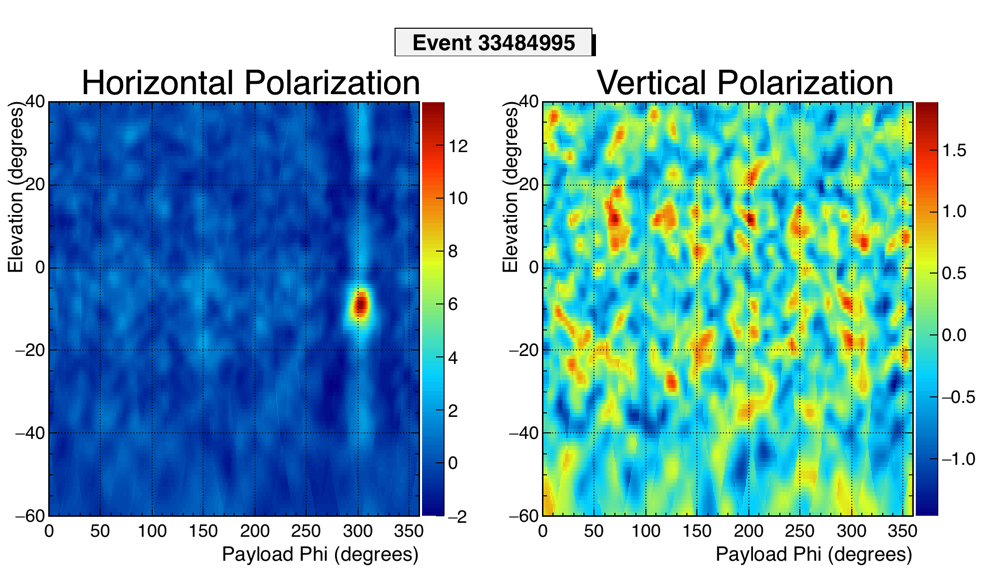
\includegraphics[width=\textwidth]{figures/intMap/intMap_ev33484995}
			\caption{Interferometric maps for event 33484995} 
		\label{fig:Ev33484995_map}
		\end{figure}			
	
		\subsubsection{Event 41529195}
		\begin{figure}
		\centering
			\includegraphics[width=\textwidth]{figures/eventStuff/Ev41529195_waveform}
			\caption{Top Coherently summed waveform.  Bottom: De-dispersed waveform} 
		\label{fig:Ev41529195_waveform}
		\end{figure}
		
		\begin{figure}
		\centering
			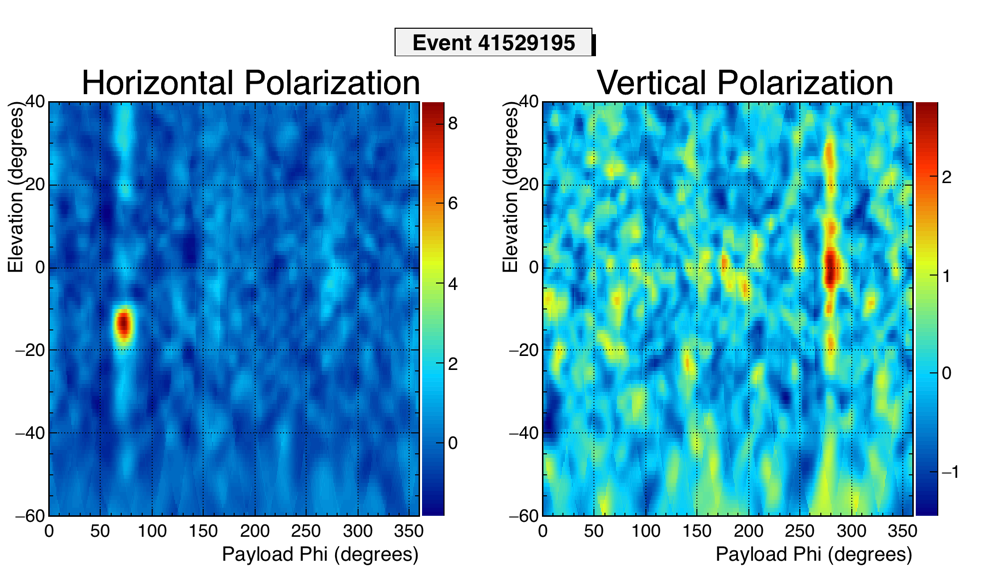
\includegraphics[width=\textwidth]{figures/intMap/intMap_ev41529195}
			\caption{Interferometric maps for event 41529195} 
		\label{fig:Ev41529195_map}
		\end{figure}			
	
		\subsubsection{Event 58592863}
		\begin{figure}
		\centering
			\includegraphics[width=\textwidth]{figures/eventStuff/Ev58592863_waveform}
			\caption{Top Coherently summed waveform.  Bottom: De-dispersed waveform} 
		\label{fig:Ev58592863_waveform}
		\end{figure}
		
		\begin{figure}
		\centering
			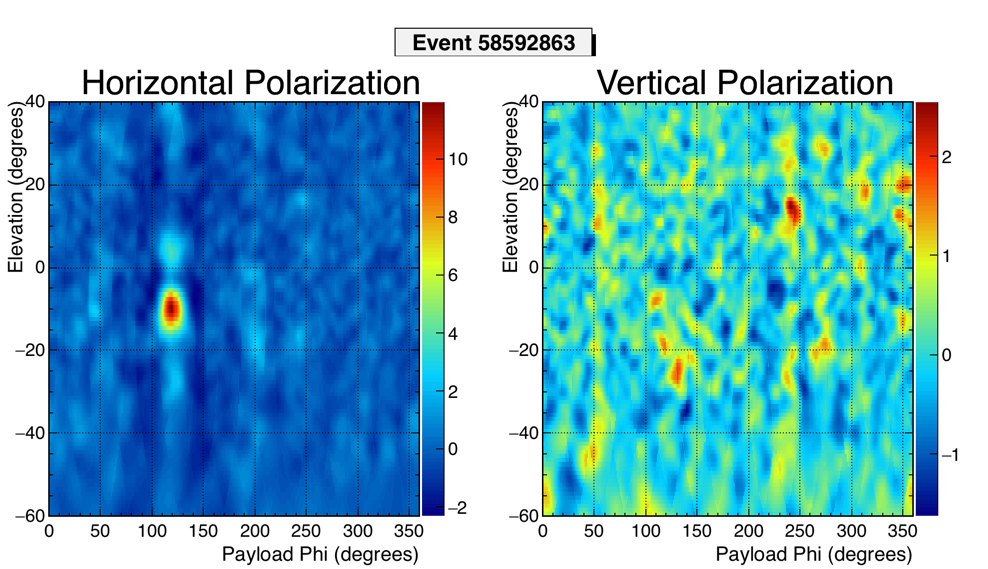
\includegraphics[width=\textwidth]{figures/intMap/intMap_ev58592863}
			\caption{Interferometric maps for event 58592863} 
		\label{fig:Ev58592863_map}
		\end{figure}			
	
		\subsubsection{Event 66313844}
		\begin{figure}
		\centering
			\includegraphics[width=\textwidth]{figures/eventStuff/Ev66313844_waveform}
			\caption{Top Coherently summed waveform.  Bottom: De-dispersed waveform} 
		\label{fig:Ev66313844_waveform}
		\end{figure}
		
		\begin{figure}
		\centering
			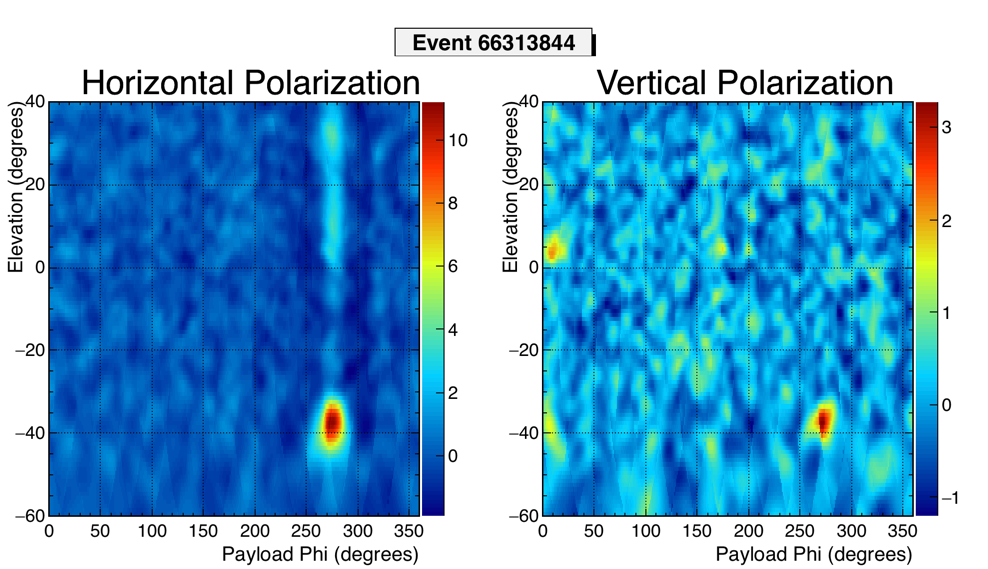
\includegraphics[width=\textwidth]{figures/intMap/intMap_ev66313844}
			\caption{Interferometric maps for event 66313844} 
		\label{fig:Ev66313844_map}
		\end{figure}			
	
		\subsubsection{Event 68298837}
		\begin{figure}
		\centering
			\includegraphics[width=\textwidth]{figures/eventStuff/Ev68298837_waveform}
			\caption{Top Coherently summed waveform.  Bottom: De-dispersed waveform} 
		\label{fig:Ev68298837_waveform}
		\end{figure}
		
		\begin{figure}
		\centering
			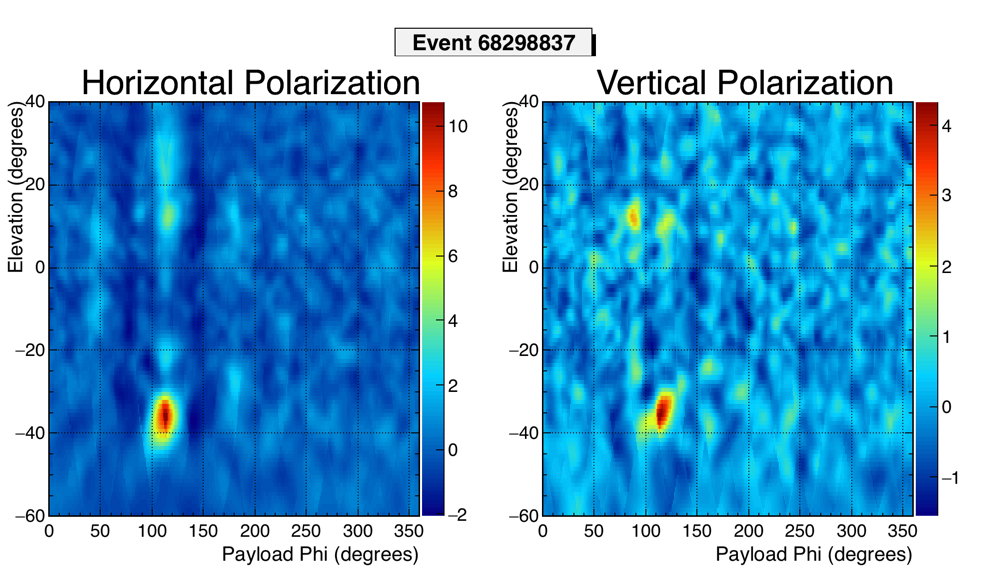
\includegraphics[width=\textwidth]{figures/intMap/intMap_ev68298837}
			\caption{Interferometric maps for event 68298837} 
		\label{fig:Ev68298837_map}
		\end{figure}			
	
		\subsubsection{Event 70013898}
		\begin{figure}
		\centering
			\includegraphics[width=\textwidth]{figures/eventStuff/Ev70013898_waveform}
			\caption{Top Coherently summed waveform.  Bottom: De-dispersed waveform} 
		\label{fig:Ev70013898_waveform}
		\end{figure}
		
		\begin{figure}
		\centering
			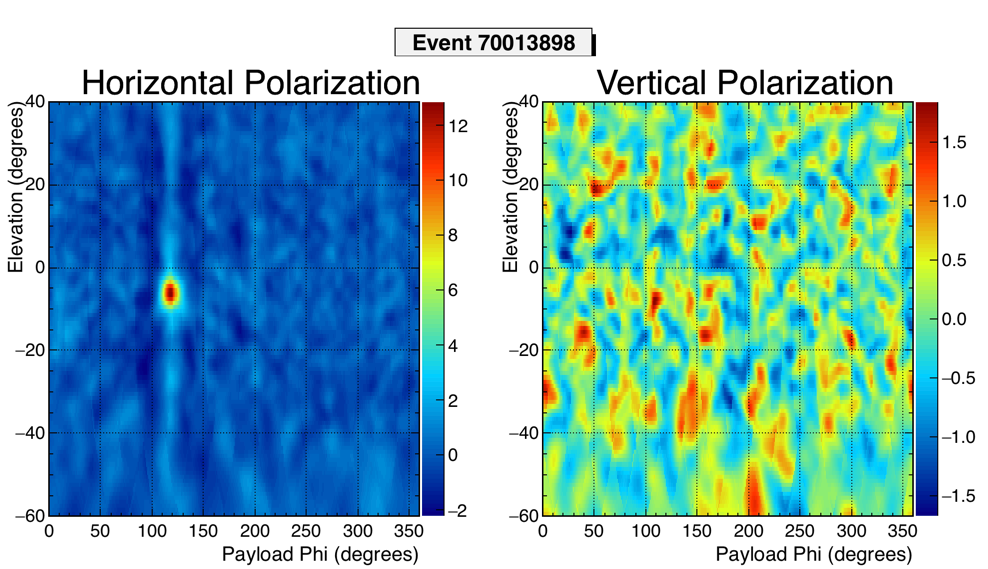
\includegraphics[width=\textwidth]{figures/intMap/intMap_ev70013898}
			\caption{Interferometric maps for event 70013898} 
		\label{fig:Ev70013898_map}
		\end{figure}			
	
		\subsubsection{Event 73726742}
		\begin{figure}
		\centering
			\includegraphics[width=\textwidth]{figures/eventStuff/Ev73726742_waveform}
			\caption{Top Coherently summed waveform.  Bottom: De-dispersed waveform} 
		\label{fig:Ev73726742_waveform}
		\end{figure}
		
		\begin{figure}
		\centering
			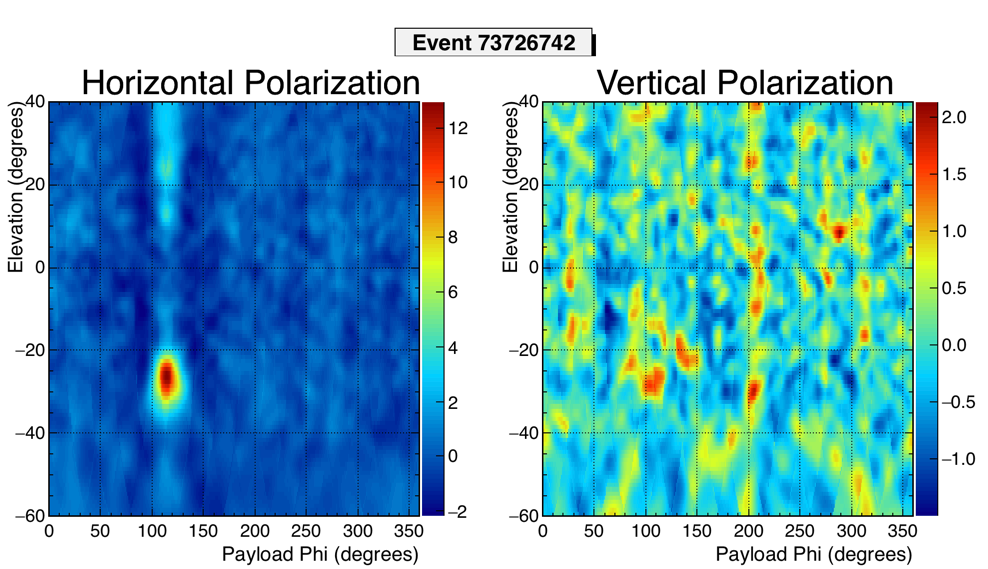
\includegraphics[width=\textwidth]{figures/intMap/intMap_ev73726742}
			\caption{Interferometric maps for event 73726742} 
		\label{fig:Ev73726742_map}
		\end{figure}			
	
		\subsubsection{Event 75277769}
		\begin{figure}
		\centering
			\includegraphics[width=\textwidth]{figures/eventStuff/Ev75277769_waveform}
			\caption{Top Coherently summed waveform.  Bottom: De-dispersed waveform} 
		\label{fig:Ev75277769_waveform}
		\end{figure}
		
		\begin{figure}
		\centering
			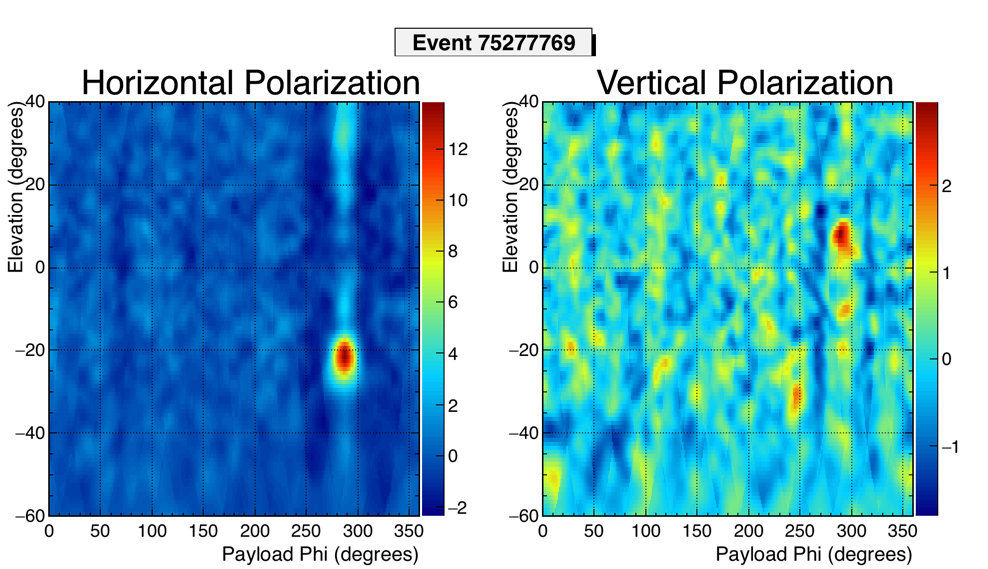
\includegraphics[width=\textwidth]{figures/intMap/intMap_ev75277769}
			\caption{Interferometric maps for event 75277769} 
		\label{fig:Ev75277769_map}
		\end{figure}			
	
		\subsubsection{Event 83877990}
		\begin{figure}
		\centering
			\includegraphics[width=\textwidth]{figures/eventStuff/Ev83877990_waveform}
			\caption{Top Coherently summed waveform.  Bottom: De-dispersed waveform} 
		\label{fig:Ev83877990_waveform}
		\end{figure}
		
		\begin{figure}
		\centering
			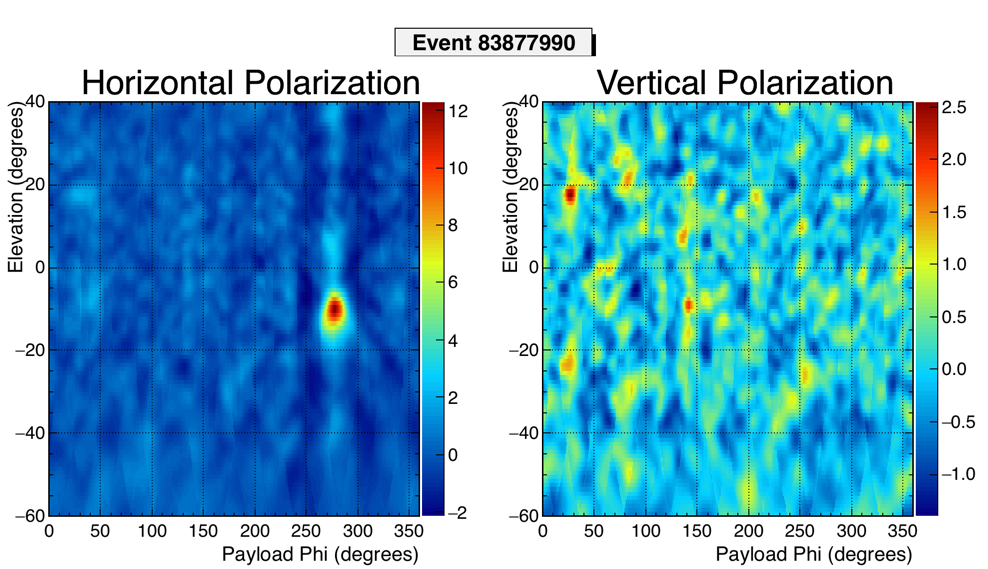
\includegraphics[width=\textwidth]{figures/intMap/intMap_ev83877990}
			\caption{Interferometric maps for event 83877990} 
		\label{fig:Ev83877990_map}
		\end{figure}			





\section{\texorpdfstring{$\nu_{\tau}$} Candidate Polarity Unblinding}
	After setting the cuts, determining the background estimate, and compiling a list of candidate events, permission to look at the results of the polarity estimator was asked of the collaboration.  The results of the unblinding are shown in Table \ref{tab:polarityUnblinding}.

	\begin{figure}
	\centering
	\begin{tabular}[c]{|c|c|c|c|}
	\hline
	Event Number & Above/Below Horizon & Coherent Polarity & Deconvolved Polarity \\
	\hline
  9097075 & Below &  0 & 0 \\
 11116669 & Below &  0 & 0 \\
 11989349 & Below &  0 & 0 \\
 \hline
 15717147 & Below &  1 & 1 \\
 \hline
 16952229 & Below &  0 & 0 \\
 19459851 & Below &  0 & 0 \\
 23695286 & Below &  0 & 0 \\
 \hline
 27142546 & Above &  1 & 1 \\
 \hline
 32907848 & Below &  0 & 0 \\
 33484995 & Below &  0 & 0 \\
 \hline
 39599205 & Above &  1 & 1 \\
 \hline
 41529195 & Below &  0 & 0 \\
 58592863 & Below &  0 & 0 \\
 62273732 & Below &  0 & 0 \\
 66313844 & Below &  0 & 0 \\
 68298837 & Below &  0 & 0 \\
 70013898 & Below &  0 & 0 \\
 73726742 & Below &  0 & 0 \\
 75277769 & Below &  0 & 0 \\
 83877990 & Below &  0 & 0 \\
 \hline
 \end{tabular}
	\caption{Results of the polarity unblinding.  Events are classified into above horizon directly observed events, or below horizon reflected events.  The value for the polarity estimate is a binary value representing the sign of the absolute peak of the highest valued simulated CR template correlation.  15 of the reflected events exhibit the same polarity, which is opposite that observed from the 2 directly observed events.  1 below horizon event is observed to have an inverted polarity.}%
\label{tab:polarityUnblinding}
\end{figure}
	
	  After unblinding the data, it was determined that 15 of the below horizon events shared the same polarity, opposite of the two above horizon events.  1 event that points below the horizon, event number 15717147, has an inverted polarity.  A plot overlaying H-pol waveforms for below horizon events, with their measured polarities, is shown in Figure \ref{fig:hPolOverlay_unblinded}.  A plot overlaying the flipped polarity below horizon event with the observed above horizon events is shown in Figure \ref{fig:directEventOverlay}.
	  
	  This flipped polarity event is consistent with a directly observed EAS shower.  The measured elevation angle of the event was 35$^\circ$ below the horizontal, well below the horizon.  A directly observed EAS shower with incident particle emerging from the ice is the expected signal from a UHE$\nu_{\tau}$.  However, additional study is required to confirm this result.
	  
		\begin{figure}
			\centering
				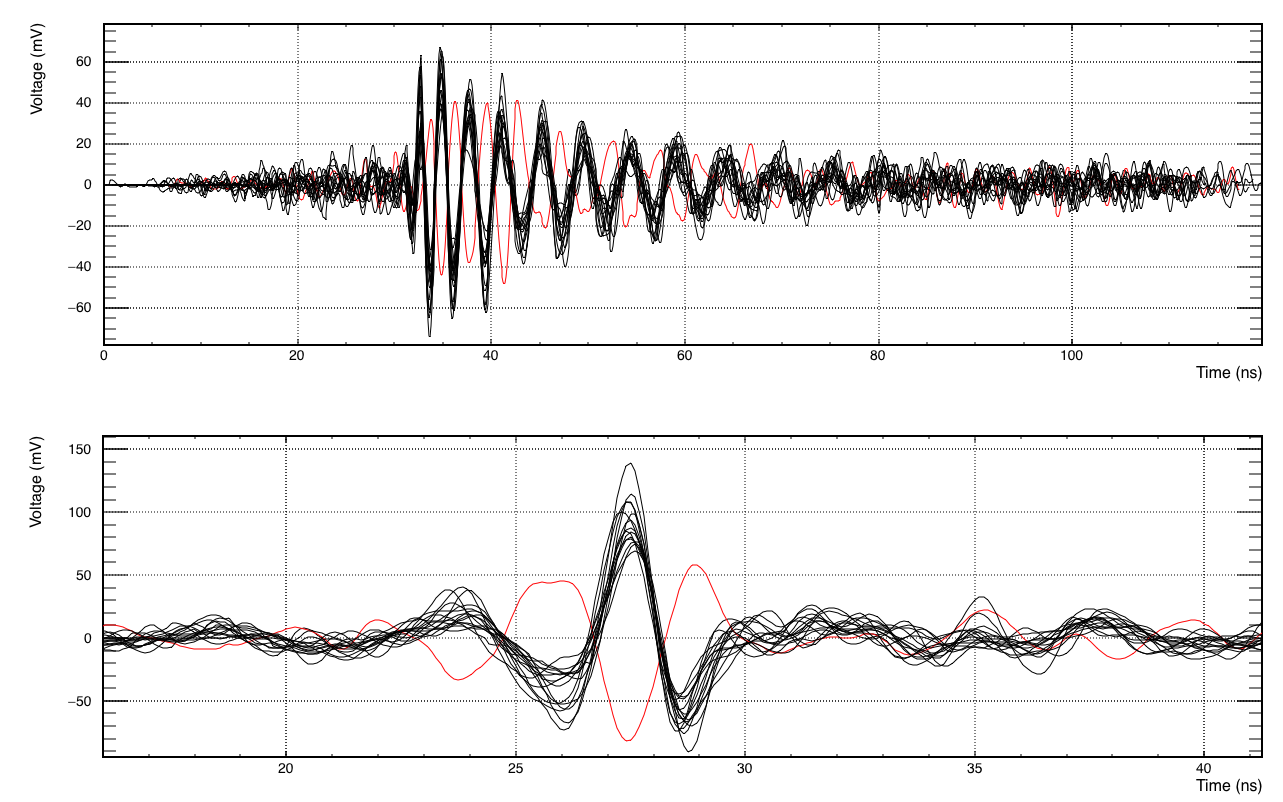
\includegraphics[width=\textwidth]{figures/hPolOverlay_unblinded}
				\caption{18 below horizon CR candidate events overlayed.  These waveforms show the true measured polarity without blinding.  They have been aligned to their peak correlation, except the flipped polarity event, which is aligned to the peak anti-correlation.  The flipped waveform is highlighted in red.  Top: Coherently summed waveform.  Bottom: All Pass Filter De-dispersed waveform. } 
			\label{fig:hPolOverlay_unblinded}
		\end{figure}		  
		
		\begin{figure}
			\centering
				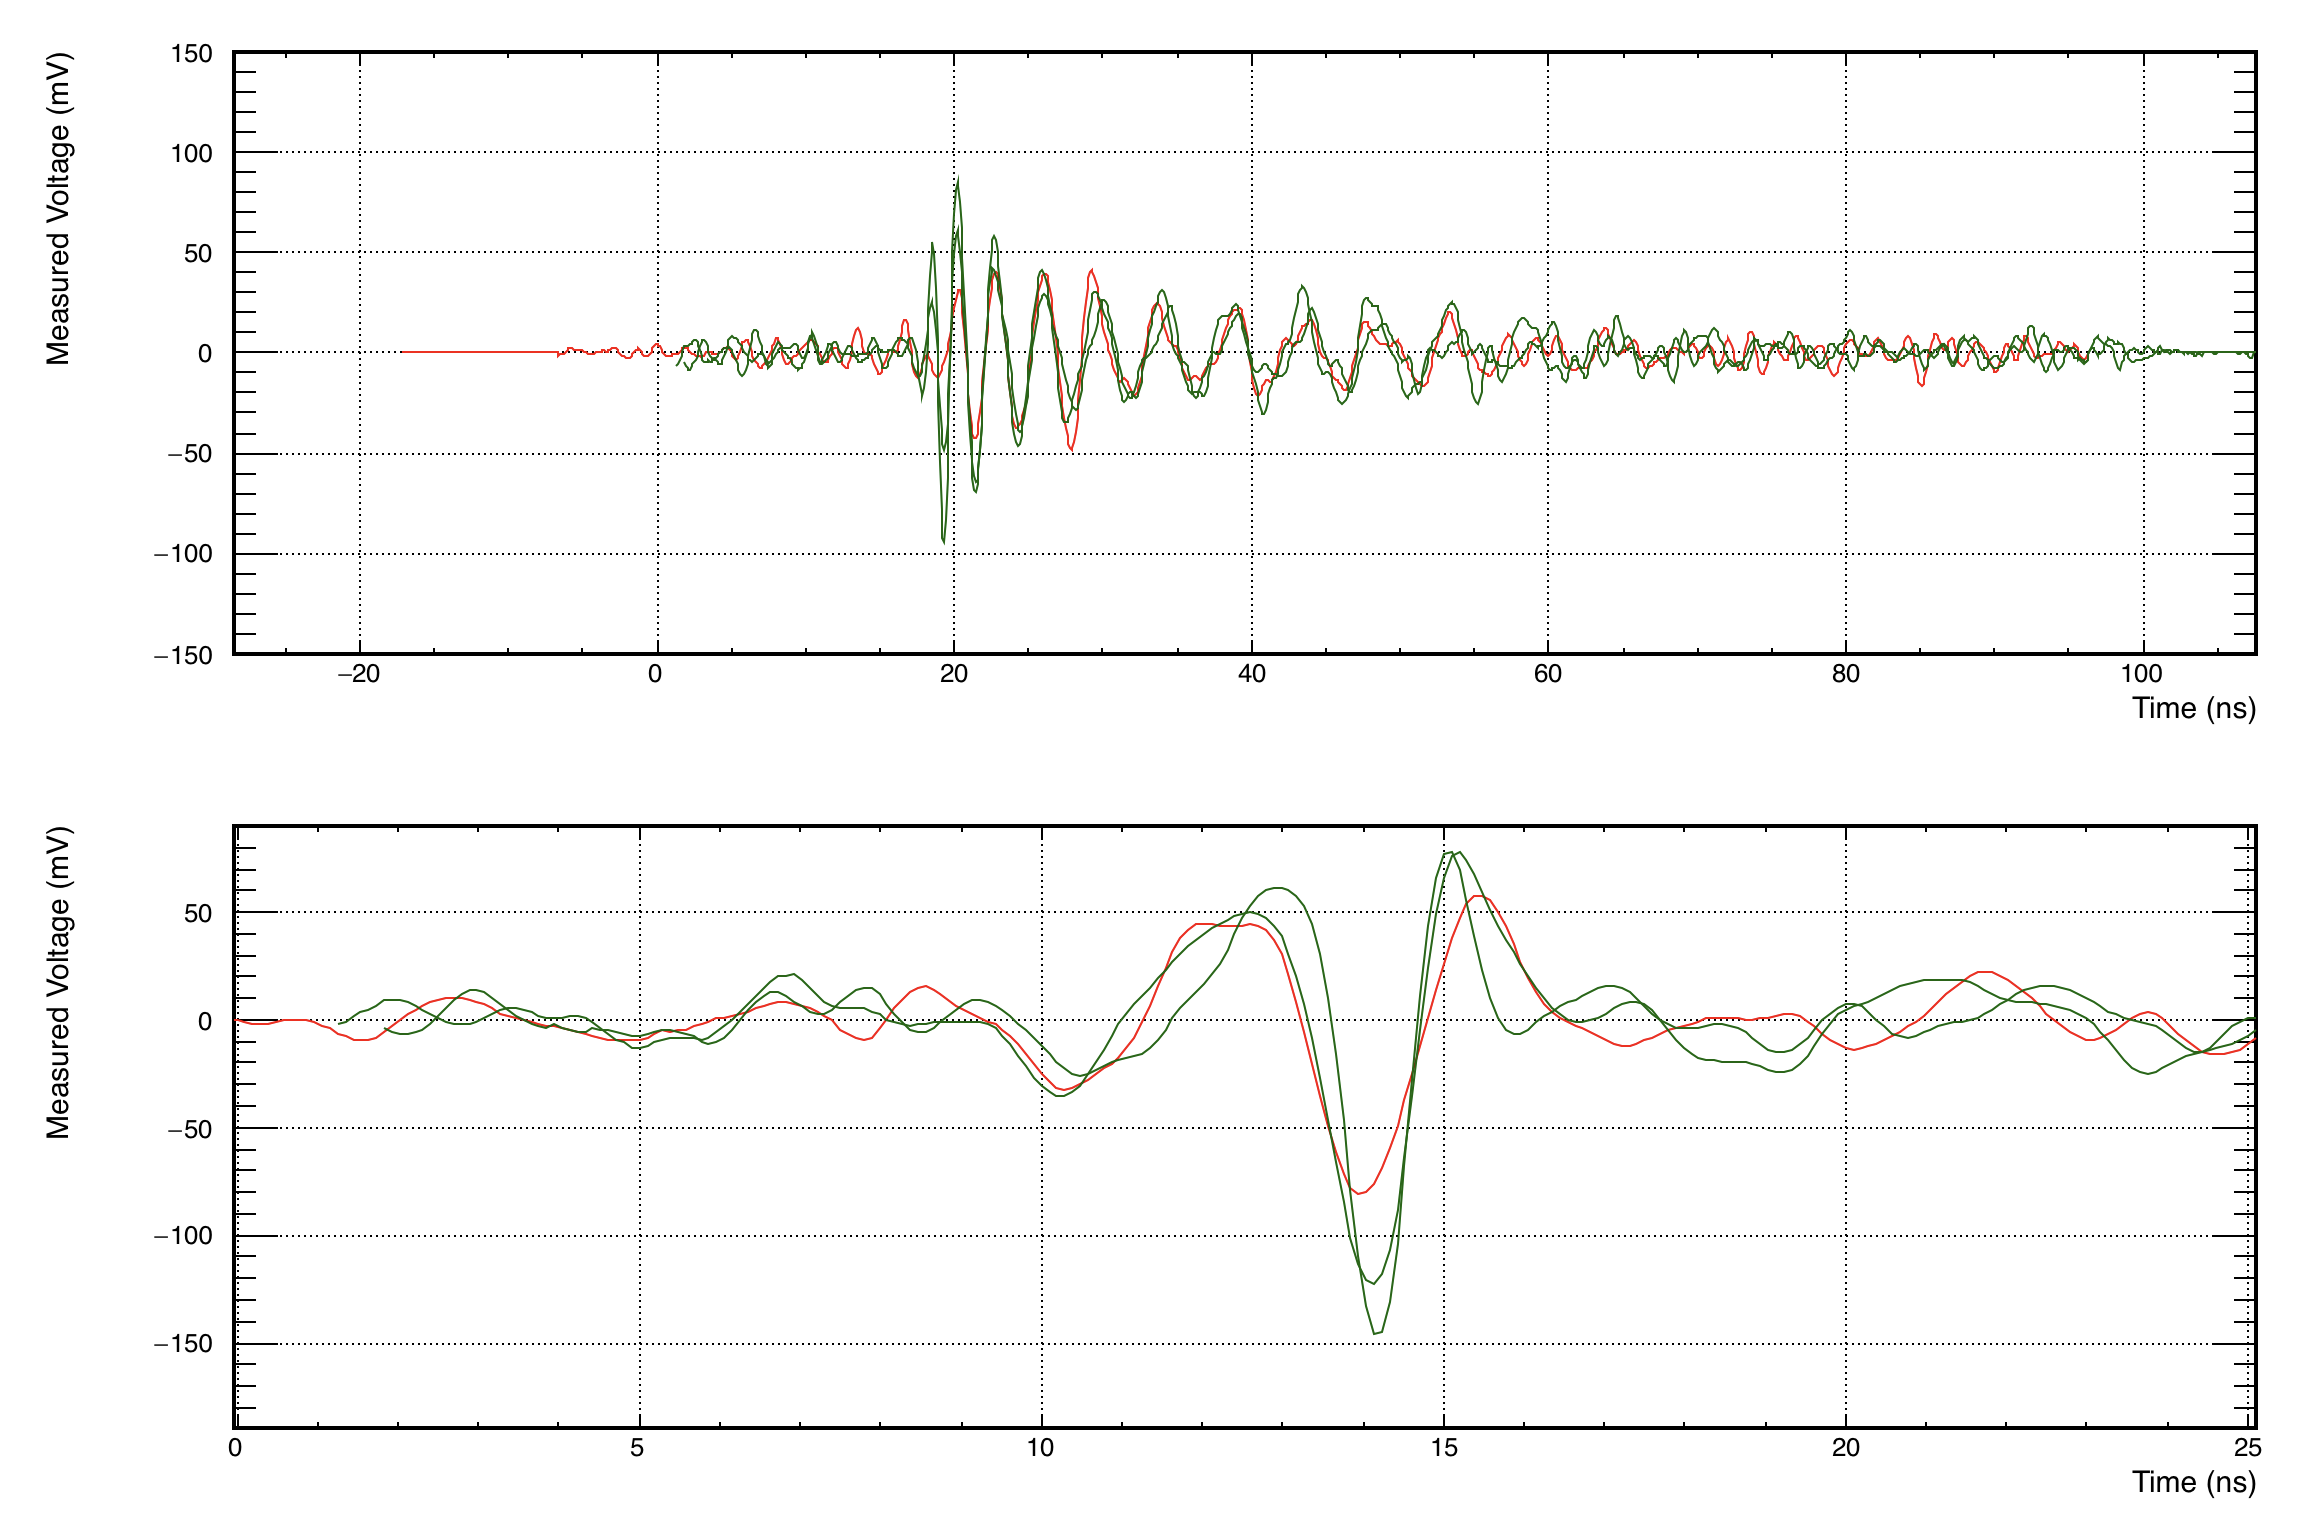
\includegraphics[width=\textwidth]{figures/directEventOverlay}
				\caption{Both above horizon CR candidate events overlaid with the one flipped polarity below horizon event.  These waveforms show the true measured polarity without blinding.  They have been aligned to their peak correlation.  The flipped waveform is highlighted in red.  Top: Coherently summed waveform.  Bottom: All Pass Filter De-dispersed waveform. } 
			\label{fig:directEventOverlay}	
		\end{figure}			
		
	
%	\subsection{Energy Estimates}


%skipping this for now
%\section{Cosmic Ray Flux Estimate}

%	\subsection{Livetime}

%	\subsection{Instrumented Volume}
	
%	\subsection{Cut Efficiency}
	

	
%\section{$\nu_{\tau}$ Flux Estimates}




%	\subsection{Bayesian Probability}
		%However, I think that using the base list to compile distributions where no events passed the impulsivity cuts is more Bayesian, since it includes an assumption that known bases cause impulsive events even if we didn't observe any impulsive events from any specific base.  